\documentclass[preprint,12pt,authoryear]{elsarticle}
% Shared preamble of main.tex, main_blind.tex and supplement.tex
\usepackage{amsmath,amssymb,amsthm}
\usepackage{graphicx}
\usepackage{booktabs}
\usepackage{threeparttable}
\usepackage{multirow}
\usepackage{algorithm}
\usepackage{algpseudocode}
\usepackage{setspace}
\usepackage[margin=1in]{geometry}
\usepackage{xr-hyper}
\usepackage[hidelinks]{hyperref}
\usepackage{xcolor}
\usepackage{bm}
\usepackage{etoolbox}
\AtBeginEnvironment{table}{\singlespacing}
\AtBeginEnvironment{algorithm}{\singlespacing}

\newtheorem{assumption}{Assumption}
\newtheorem{proposition}{Proposition}
\newtheorem{lemma}{Lemma}
\newtheorem{remark}{Remark}
\newcommand{\E}{\mathbb{E}}
\newcommand{\M}{\mathcal{M}}
\DeclareMathOperator*{\argmin}{arg\,min}
\makeatletter
\newcommand{\nm}[1]{\ifcsname nm:#1\endcsname\csname nm:#1\endcsname\else\PackageError{numbers}{Unknown number #1}{}\fi}
\expandafter\def\csname nm:nobs\endcsname{4{,}075}
\expandafter\def\csname nm:ncty\endcsname{149}
\expandafter\def\csname nm:nobscommon\endcsname{3{,}787}
\expandafter\def\csname nm:nctycommon\endcsname{141}
\expandafter\def\csname nm:nobsunt\endcsname{4{,}157}
\expandafter\def\csname nm:nctyunt\endcsname{149}
\expandafter\def\csname nm:nobsuns\endcsname{4{,}081}
\expandafter\def\csname nm:npwtten\endcsname{2{,}658}
\expandafter\def\csname nm:nctypwtten\endcsname{115}
\expandafter\def\csname nm:npwtel\endcsname{3{,}178}
\expandafter\def\csname nm:nctypwtel\endcsname{118}
\expandafter\def\csname nm:nnopre\endcsname{1}
\expandafter\def\csname nm:nopre\endcsname{Montenegro}
\expandafter\def\csname nm:covhi\endcsname{53}
\expandafter\def\csname nm:tothi\endcsname{86}
\expandafter\def\csname nm:covum\endcsname{45}
\expandafter\def\csname nm:totum\endcsname{59}
\expandafter\def\csname nm:covlm\endcsname{37}
\expandafter\def\csname nm:totlm\endcsname{47}
\expandafter\def\csname nm:covli\endcsname{14}
\expandafter\def\csname nm:totli\endcsname{25}
\expandafter\def\csname nm:nflags\endcsname{39}
\expandafter\def\csname nm:flagsmobile\endcsname{18}
\expandafter\def\csname nm:flagsbroadband\endcsname{13}
\expandafter\def\csname nm:flagsinternet\endcsname{8}
\expandafter\def\csname nm:fedml\endcsname{-2.64}
\expandafter\def\csname nm:fedmlse\endcsname{1.33}
\expandafter\def\csname nm:fedmlten\endcsname{-0.264}
\expandafter\def\csname nm:cilo\endcsname{-0.524}
\expandafter\def\csname nm:cihi\endcsname{-0.004}
\expandafter\def\csname nm:twse\endcsname{1.40}
\expandafter\def\csname nm:cihitw\endcsname{0.009}
\expandafter\def\csname nm:cilotw\endcsname{-0.538}
\expandafter\def\csname nm:twfe\endcsname{-2.84}
\expandafter\def\csname nm:twfese\endcsname{0.79}
\expandafter\def\csname nm:tbten\endcsname{-0.284}
\expandafter\def\csname nm:savg\endcsname{-2.59}
\expandafter\def\csname nm:savgse\endcsname{1.51}
\expandafter\def\csname nm:rise\endcsname{71}
\expandafter\def\csname nm:riseimpl\endcsname{-1.9}
\expandafter\def\csname nm:riseimplhi\endcsname{-0.03}
\expandafter\def\csname nm:idvar\endcsname{0.22}
\expandafter\def\csname nm:idvartot\endcsname{2.5}
\expandafter\def\csname nm:idvarlowA\endcsname{0.11}
\expandafter\def\csname nm:idvarlowB\endcsname{0.14}
\expandafter\def\csname nm:dmedlowA\endcsname{0.04}
\expandafter\def\csname nm:dmedlowB\endcsname{0.07}
\expandafter\def\csname nm:common\endcsname{-2.44}
\expandafter\def\csname nm:commonse\endcsname{1.22}
\expandafter\def\csname nm:commonn\endcsname{3{,}787}
\expandafter\def\csname nm:commondiffA\endcsname{-3.55}
\expandafter\def\csname nm:commondiffAse\endcsname{3.36}
\expandafter\def\csname nm:rf\endcsname{-3.15}
\expandafter\def\csname nm:rfse\endcsname{1.22}
\expandafter\def\csname nm:rfn\endcsname{4{,}075}
\expandafter\def\csname nm:rfdiffA\endcsname{0.19}
\expandafter\def\csname nm:rfdiffAse\endcsname{2.89}
\expandafter\def\csname nm:ry\endcsname{-2.55}
\expandafter\def\csname nm:ryse\endcsname{1.32}
\expandafter\def\csname nm:ryn\endcsname{4{,}075}
\expandafter\def\csname nm:rydiffA\endcsname{-0.33}
\expandafter\def\csname nm:rydiffAse\endcsname{3.68}
\expandafter\def\csname nm:precovid\endcsname{-3.35}
\expandafter\def\csname nm:precovidse\endcsname{1.45}
\expandafter\def\csname nm:precovidn\endcsname{3{,}244}
\expandafter\def\csname nm:precoviddiffA\endcsname{-1.78}
\expandafter\def\csname nm:precoviddiffAse\endcsname{4.39}
\expandafter\def\csname nm:nocovid\endcsname{-2.93}
\expandafter\def\csname nm:nocovidse\endcsname{1.33}
\expandafter\def\csname nm:nocovidn\endcsname{3{,}800}
\expandafter\def\csname nm:nocoviddiffA\endcsname{0.43}
\expandafter\def\csname nm:nocoviddiffAse\endcsname{3.89}
\expandafter\def\csname nm:gdppc\endcsname{-3.02}
\expandafter\def\csname nm:gdppcse\endcsname{1.36}
\expandafter\def\csname nm:gdppcn\endcsname{4{,}075}
\expandafter\def\csname nm:gdppcdiffA\endcsname{0.44}
\expandafter\def\csname nm:gdppcdiffAse\endcsname{3.68}
\expandafter\def\csname nm:spi\endcsname{-2.24}
\expandafter\def\csname nm:spise\endcsname{1.34}
\expandafter\def\csname nm:spin\endcsname{2{,}147}
\expandafter\def\csname nm:spidiffA\endcsname{-0.28}
\expandafter\def\csname nm:spidiffAse\endcsname{3.24}
\expandafter\def\csname nm:pwtel\endcsname{-2.60}
\expandafter\def\csname nm:pwtelse\endcsname{1.33}
\expandafter\def\csname nm:pwteln\endcsname{3{,}178}
\expandafter\def\csname nm:pwteldiffA\endcsname{11.14}
\expandafter\def\csname nm:pwteldiffAse\endcsname{6.19}
\expandafter\def\csname nm:pwtten\endcsname{-2.12}
\expandafter\def\csname nm:pwttense\endcsname{1.54}
\expandafter\def\csname nm:pwttenn\endcsname{2{,}658}
\expandafter\def\csname nm:pwttendiffA\endcsname{8.00}
\expandafter\def\csname nm:pwttendiffAse\endcsname{5.87}
\expandafter\def\csname nm:mobbb\endcsname{-0.50}
\expandafter\def\csname nm:mobbbse\endcsname{1.24}
\expandafter\def\csname nm:mobbbn\endcsname{3{,}977}
\expandafter\def\csname nm:mobbbdiffA\endcsname{1.62}
\expandafter\def\csname nm:mobbbdiffAse\endcsname{3.02}
\expandafter\def\csname nm:mobbbnf\endcsname{-1.24}
\expandafter\def\csname nm:mobbbnfse\endcsname{1.33}
\expandafter\def\csname nm:mobbbnfn\endcsname{3{,}086}
\expandafter\def\csname nm:mobbbnfdiffA\endcsname{6.44}
\expandafter\def\csname nm:mobbbnfdiffAse\endcsname{3.00}
\expandafter\def\csname nm:orig\endcsname{-0.69}
\expandafter\def\csname nm:origse\endcsname{1.18}
\expandafter\def\csname nm:orign\endcsname{3{,}949}
\expandafter\def\csname nm:origdiffA\endcsname{2.67}
\expandafter\def\csname nm:origdiffAse\endcsname{2.88}
\expandafter\def\csname nm:ict\endcsname{-3.03}
\expandafter\def\csname nm:ictse\endcsname{1.56}
\expandafter\def\csname nm:ictn\endcsname{3{,}977}
\expandafter\def\csname nm:ictdiffA\endcsname{-2.13}
\expandafter\def\csname nm:ictdiffAse\endcsname{4.52}
\expandafter\def\csname nm:nores\endcsname{-2.17}
\expandafter\def\csname nm:noresse\endcsname{1.39}
\expandafter\def\csname nm:noresn\endcsname{3{,}199}
\expandafter\def\csname nm:noresdiffA\endcsname{0.68}
\expandafter\def\csname nm:noresdiffAse\endcsname{3.38}
\expandafter\def\csname nm:popw\endcsname{-2.71}
\expandafter\def\csname nm:popwse\endcsname{1.29}
\expandafter\def\csname nm:popwn\endcsname{4{,}075}
\expandafter\def\csname nm:popwdiffA\endcsname{-0.47}
\expandafter\def\csname nm:popwdiffAse\endcsname{3.53}
\expandafter\def\csname nm:unt\endcsname{-3.25}
\expandafter\def\csname nm:untse\endcsname{1.58}
\expandafter\def\csname nm:untn\endcsname{4{,}157}
\expandafter\def\csname nm:untdiffA\endcsname{-0.12}
\expandafter\def\csname nm:untdiffAse\endcsname{4.21}
\expandafter\def\csname nm:uns\endcsname{-2.71}
\expandafter\def\csname nm:unsse\endcsname{1.29}
\expandafter\def\csname nm:unsn\endcsname{4{,}081}
\expandafter\def\csname nm:unsdiffA\endcsname{-1.05}
\expandafter\def\csname nm:unsdiffAse\endcsname{3.56}
\expandafter\def\csname nm:nomund\endcsname{-2.46}
\expandafter\def\csname nm:nomundse\endcsname{1.10}
\expandafter\def\csname nm:nomundn\endcsname{4{,}075}
\expandafter\def\csname nm:nomunddiffA\endcsname{-0.91}
\expandafter\def\csname nm:nomunddiffAse\endcsname{2.55}
\expandafter\def\csname nm:invest\endcsname{-2.51}
\expandafter\def\csname nm:investse\endcsname{1.36}
\expandafter\def\csname nm:investn\endcsname{4{,}047}
\expandafter\def\csname nm:investdiffA\endcsname{-1.54}
\expandafter\def\csname nm:investdiffAse\endcsname{3.71}
\expandafter\def\csname nm:lagtwo\endcsname{-2.31}
\expandafter\def\csname nm:lagtwose\endcsname{1.30}
\expandafter\def\csname nm:lagtwon\endcsname{4{,}005}
\expandafter\def\csname nm:lagtwodiffA\endcsname{-0.16}
\expandafter\def\csname nm:lagtwodiffAse\endcsname{3.89}
\expandafter\def\csname nm:popwavg\endcsname{-2.63}
\expandafter\def\csname nm:popwavgse\endcsname{1.67}
\expandafter\def\csname nm:diffA\endcsname{-0.70}
\expandafter\def\csname nm:diffseA\endcsname{3.60}
\expandafter\def\csname nm:blpA\endcsname{-0.10}
\expandafter\def\csname nm:blpseA\endcsname{0.49}
\expandafter\def\csname nm:gatelowA\endcsname{-2.15}
\expandafter\def\csname nm:gatelowseA\endcsname{3.00}
\expandafter\def\csname nm:gatehighA\endcsname{-2.72}
\expandafter\def\csname nm:gatehighseA\endcsname{1.65}
\expandafter\def\csname nm:gatemidA\endcsname{-2.63}
\expandafter\def\csname nm:gatemidseA\endcsname{1.44}
\expandafter\def\csname nm:diffx5A\endcsname{-0.63}
\expandafter\def\csname nm:diffx5seA\endcsname{3.36}
\expandafter\def\csname nm:pconstA\endcsname{0.96}
\expandafter\def\csname nm:pconstAeq\endcsname{=0.96}
\expandafter\def\csname nm:plinA\endcsname{0.85}
\expandafter\def\csname nm:plinAeq\endcsname{=0.85}
\expandafter\def\csname nm:pconstuA\endcsname{0.57}
\expandafter\def\csname nm:pconstuAeq\endcsname{=0.57}
\expandafter\def\csname nm:lamA\endcsname{562}
\expandafter\def\csname nm:edfA\endcsname{2.0}
\expandafter\def\csname nm:mdeA\endcsname{1.01}
\expandafter\def\csname nm:ciloA\endcsname{-0.78}
\expandafter\def\csname nm:cihiA\endcsname{0.64}
\expandafter\def\csname nm:diffsetwA\endcsname{3.49}
\expandafter\def\csname nm:commondiffseA\endcsname{3.36}
\expandafter\def\csname nm:commonpA\endcsname{0.40}
\expandafter\def\csname nm:rydiffseA\endcsname{3.68}
\expandafter\def\csname nm:rypA\endcsname{0.97}
\expandafter\def\csname nm:rfdiffseA\endcsname{2.89}
\expandafter\def\csname nm:mobbbdiffseA\endcsname{3.02}
\expandafter\def\csname nm:precoviddiffseA\endcsname{4.39}
\expandafter\def\csname nm:diffB\endcsname{-0.76}
\expandafter\def\csname nm:diffseB\endcsname{3.27}
\expandafter\def\csname nm:blpB\endcsname{-0.81}
\expandafter\def\csname nm:blpseB\endcsname{1.40}
\expandafter\def\csname nm:gatelowB\endcsname{-0.59}
\expandafter\def\csname nm:gatelowseB\endcsname{3.00}
\expandafter\def\csname nm:gatehighB\endcsname{-1.27}
\expandafter\def\csname nm:gatehighseB\endcsname{1.43}
\expandafter\def\csname nm:gatemidB\endcsname{-4.79}
\expandafter\def\csname nm:gatemidseB\endcsname{1.81}
\expandafter\def\csname nm:diffx5B\endcsname{0.40}
\expandafter\def\csname nm:diffx5seB\endcsname{3.15}
\expandafter\def\csname nm:pconstB\endcsname{0.16}
\expandafter\def\csname nm:pconstBeq\endcsname{=0.16}
\expandafter\def\csname nm:plinB\endcsname{0.09}
\expandafter\def\csname nm:plinBeq\endcsname{=0.09}
\expandafter\def\csname nm:pconstuB\endcsname{0.04}
\expandafter\def\csname nm:pconstuBeq\endcsname{=0.04}
\expandafter\def\csname nm:lamB\endcsname{1}
\expandafter\def\csname nm:edfB\endcsname{4.0}
\expandafter\def\csname nm:mdeB\endcsname{0.92}
\expandafter\def\csname nm:ciloB\endcsname{-0.72}
\expandafter\def\csname nm:cihiB\endcsname{0.56}
\expandafter\def\csname nm:diffsetwB\endcsname{3.35}
\expandafter\def\csname nm:commondiffB\endcsname{-1.10}
\expandafter\def\csname nm:commondiffseB\endcsname{3.18}
\expandafter\def\csname nm:commonpB\endcsname{0.68}
\expandafter\def\csname nm:rydiffB\endcsname{0.19}
\expandafter\def\csname nm:rydiffseB\endcsname{3.25}
\expandafter\def\csname nm:rypB\endcsname{0.21}
\expandafter\def\csname nm:rfdiffB\endcsname{0.28}
\expandafter\def\csname nm:rfdiffseB\endcsname{2.75}
\expandafter\def\csname nm:mobbbdiffB\endcsname{0.01}
\expandafter\def\csname nm:mobbbdiffseB\endcsname{2.60}
\expandafter\def\csname nm:precoviddiffB\endcsname{0.88}
\expandafter\def\csname nm:precoviddiffseB\endcsname{4.58}
\expandafter\def\csname nm:diffC\endcsname{-0.11}
\expandafter\def\csname nm:diffseC\endcsname{11.17}
\expandafter\def\csname nm:blpC\endcsname{-0.28}
\expandafter\def\csname nm:blpseC\endcsname{0.57}
\expandafter\def\csname nm:gatelowC\endcsname{-0.26}
\expandafter\def\csname nm:gatelowseC\endcsname{11.14}
\expandafter\def\csname nm:gatehighC\endcsname{-0.74}
\expandafter\def\csname nm:gatehighseC\endcsname{1.63}
\expandafter\def\csname nm:gatemidC\endcsname{-3.18}
\expandafter\def\csname nm:gatemidseC\endcsname{1.67}
\expandafter\def\csname nm:diffx5C\endcsname{6.96}
\expandafter\def\csname nm:diffx5seC\endcsname{8.48}
\expandafter\def\csname nm:pconstC\endcsname{0.09}
\expandafter\def\csname nm:pconstCeq\endcsname{=0.09}
\expandafter\def\csname nm:plinC\endcsname{0.16}
\expandafter\def\csname nm:plinCeq\endcsname{=0.16}
\expandafter\def\csname nm:pconstuC\endcsname{0.03}
\expandafter\def\csname nm:pconstuCeq\endcsname{=0.03}
\expandafter\def\csname nm:lamC\endcsname{0.0316}
\expandafter\def\csname nm:edfC\endcsname{5.9}
\expandafter\def\csname nm:mdeC\endcsname{3.13}
\expandafter\def\csname nm:ciloC\endcsname{-2.20}
\expandafter\def\csname nm:cihiC\endcsname{2.18}
\expandafter\def\csname nm:diffsetwC\endcsname{10.62}
\expandafter\def\csname nm:commondiffC\endcsname{5.72}
\expandafter\def\csname nm:commondiffseC\endcsname{4.88}
\expandafter\def\csname nm:commonpC\endcsname{0.49}
\expandafter\def\csname nm:rydiffC\endcsname{-2.71}
\expandafter\def\csname nm:rydiffseC\endcsname{10.55}
\expandafter\def\csname nm:rypC\endcsname{0.17}
\expandafter\def\csname nm:rfdiffC\endcsname{-8.00}
\expandafter\def\csname nm:rfdiffseC\endcsname{13.31}
\expandafter\def\csname nm:mobbbdiffC\endcsname{2.45}
\expandafter\def\csname nm:mobbbdiffseC\endcsname{4.22}
\expandafter\def\csname nm:precoviddiffC\endcsname{7.04}
\expandafter\def\csname nm:precoviddiffseC\endcsname{5.09}
\expandafter\def\csname nm:laysdiff\endcsname{0.44}
\expandafter\def\csname nm:laysdiffse\endcsname{3.46}
\expandafter\def\csname nm:laysp\endcsname{0.96}
\expandafter\def\csname nm:layspeq\endcsname{=0.96}
\expandafter\def\csname nm:layslow\endcsname{-3.08}
\expandafter\def\csname nm:layslowse\endcsname{2.88}
\expandafter\def\csname nm:ictBdiff\endcsname{5.54}
\expandafter\def\csname nm:ictBdiffse\endcsname{3.31}
\expandafter\def\csname nm:ictBp\endcsname{0.09}
\expandafter\def\csname nm:ictBpeq\endcsname{=0.09}
\expandafter\def\csname nm:ictBlow\endcsname{-6.45}
\expandafter\def\csname nm:ictBlowse\endcsname{3.01}
\expandafter\def\csname nm:distusdiff\endcsname{-5.16}
\expandafter\def\csname nm:distusdiffse\endcsname{2.88}
\expandafter\def\csname nm:distusp\endcsname{0.11}
\expandafter\def\csname nm:distuspeq\endcsname{=0.11}
\expandafter\def\csname nm:distuslow\endcsname{3.82}
\expandafter\def\csname nm:distuslowse\endcsname{2.66}
\expandafter\def\csname nm:presmpdiff\endcsname{0.00}
\expandafter\def\csname nm:presmpdiffse\endcsname{3.20}
\expandafter\def\csname nm:presmpp\endcsname{0.24}
\expandafter\def\csname nm:presmppeq\endcsname{=0.24}
\expandafter\def\csname nm:presmplow\endcsname{-1.42}
\expandafter\def\csname nm:presmplowse\endcsname{2.74}
\expandafter\def\csname nm:yprediff\endcsname{4.95}
\expandafter\def\csname nm:yprediffse\endcsname{3.02}
\expandafter\def\csname nm:yprep\endcsname{0.19}
\expandafter\def\csname nm:yprepeq\endcsname{=0.19}
\expandafter\def\csname nm:yprelow\endcsname{-4.62}
\expandafter\def\csname nm:yprelowse\endcsname{2.34}
\expandafter\def\csname nm:pwtelBdiff\endcsname{14.68}
\expandafter\def\csname nm:pwtelBdiffse\endcsname{3.88}
\expandafter\def\csname nm:pwtelBp\endcsname{0.000}
\expandafter\def\csname nm:pwtelBpeq\endcsname{<0.001}
\expandafter\def\csname nm:pwtelBlow\endcsname{-12.09}
\expandafter\def\csname nm:pwtelBlowse\endcsname{3.52}
\expandafter\def\csname nm:pwtelnineBdiff\endcsname{7.73}
\expandafter\def\csname nm:pwtelnineBdiffse\endcsname{4.88}
\expandafter\def\csname nm:pwtelnineBp\endcsname{0.12}
\expandafter\def\csname nm:pwtelnineBpeq\endcsname{=0.12}
\expandafter\def\csname nm:pwtelnineBlow\endcsname{-6.25}
\expandafter\def\csname nm:pwtelnineBlowse\endcsname{4.16}
\expandafter\def\csname nm:pwttenBdiff\endcsname{14.42}
\expandafter\def\csname nm:pwttenBdiffse\endcsname{4.92}
\expandafter\def\csname nm:pwttenBp\endcsname{0.008}
\expandafter\def\csname nm:pwttenBpeq\endcsname{=0.008}
\expandafter\def\csname nm:pwttenBlow\endcsname{-12.19}
\expandafter\def\csname nm:pwttenBlowse\endcsname{3.83}
\expandafter\def\csname nm:wdipwtBdiff\endcsname{2.01}
\expandafter\def\csname nm:wdipwtBdiffse\endcsname{3.55}
\expandafter\def\csname nm:wdipwtBp\endcsname{0.61}
\expandafter\def\csname nm:wdipwtBpeq\endcsname{=0.61}
\expandafter\def\csname nm:wdipwtBlow\endcsname{-5.17}
\expandafter\def\csname nm:wdipwtBlowse\endcsname{2.69}
\expandafter\def\csname nm:pwtelnaBdiff\endcsname{8.21}
\expandafter\def\csname nm:pwtelnaBdiffse\endcsname{3.42}
\expandafter\def\csname nm:pwtelnaBp\endcsname{0.08}
\expandafter\def\csname nm:pwtelnaBpeq\endcsname{=0.08}
\expandafter\def\csname nm:pwtelnaBlow\endcsname{-7.77}
\expandafter\def\csname nm:pwtelnaBlowse\endcsname{3.02}
\expandafter\def\csname nm:pwttennaBdiff\endcsname{12.21}
\expandafter\def\csname nm:pwttennaBdiffse\endcsname{4.17}
\expandafter\def\csname nm:pwttennaBp\endcsname{0.007}
\expandafter\def\csname nm:pwttennaBpeq\endcsname{=0.007}
\expandafter\def\csname nm:pwttennaBlow\endcsname{-10.62}
\expandafter\def\csname nm:pwttennaBlowse\endcsname{3.33}
\expandafter\def\csname nm:pwtelAdiff\endcsname{11.14}
\expandafter\def\csname nm:pwtelAdiffse\endcsname{6.19}
\expandafter\def\csname nm:pwtelAp\endcsname{0.22}
\expandafter\def\csname nm:pwtelApeq\endcsname{=0.22}
\expandafter\def\csname nm:pwtelAlow\endcsname{-11.56}
\expandafter\def\csname nm:pwtelAlowse\endcsname{6.07}
\expandafter\def\csname nm:pwttenAdiff\endcsname{8.00}
\expandafter\def\csname nm:pwttenAdiffse\endcsname{5.87}
\expandafter\def\csname nm:pwttenAp\endcsname{0.04}
\expandafter\def\csname nm:pwttenApeq\endcsname{=0.04}
\expandafter\def\csname nm:pwttenAlow\endcsname{-10.32}
\expandafter\def\csname nm:pwttenAlowse\endcsname{5.69}
\expandafter\def\csname nm:twgl\endcsname{1.77}
\expandafter\def\csname nm:twglse\endcsname{0.85}
\expandafter\def\csname nm:twgs\endcsname{3.90}
\expandafter\def\csname nm:twgsse\endcsname{1.14}
\expandafter\def\csname nm:twgh\endcsname{-0.58}
\expandafter\def\csname nm:twghse\endcsname{1.04}
\expandafter\def\csname nm:holmA\endcsname{0.96}
\expandafter\def\csname nm:holmAeq\endcsname{=0.96}
\expandafter\def\csname nm:holmuA\endcsname{0.57}
\expandafter\def\csname nm:holmuAeq\endcsname{=0.57}
\expandafter\def\csname nm:holmlinA\endcsname{0.85}
\expandafter\def\csname nm:holmlinAeq\endcsname{=0.85}
\expandafter\def\csname nm:holmB\endcsname{0.33}
\expandafter\def\csname nm:holmBeq\endcsname{=0.33}
\expandafter\def\csname nm:holmuB\endcsname{0.10}
\expandafter\def\csname nm:holmuBeq\endcsname{=0.10}
\expandafter\def\csname nm:holmlinB\endcsname{0.27}
\expandafter\def\csname nm:holmlinBeq\endcsname{=0.27}
\expandafter\def\csname nm:holmC\endcsname{0.28}
\expandafter\def\csname nm:holmCeq\endcsname{=0.28}
\expandafter\def\csname nm:holmuC\endcsname{0.10}
\expandafter\def\csname nm:holmuCeq\endcsname{=0.10}
\expandafter\def\csname nm:holmlinC\endcsname{0.32}
\expandafter\def\csname nm:holmlinCeq\endcsname{=0.32}
\expandafter\def\csname nm:pdose\endcsname{0.14}
\expandafter\def\csname nm:pdoseeq\endcsname{=0.14}
\expandafter\def\csname nm:pdoseu\endcsname{0.98}
\expandafter\def\csname nm:pdoseueq\endcsname{=0.98}
\expandafter\def\csname nm:dosestart\endcsname{13}
\expandafter\def\csname nm:lpa\endcsname{-0.27}
\expandafter\def\csname nm:lpsea\endcsname{0.13}
\expandafter\def\csname nm:lpca\endcsname{-0.43}
\expandafter\def\csname nm:lpcsea\endcsname{0.16}
\expandafter\def\csname nm:lpna\endcsname{4{,}075}
\expandafter\def\csname nm:lpdiffa\endcsname{-0.67}
\expandafter\def\csname nm:lpdiffsea\endcsname{3.23}
\expandafter\def\csname nm:lpb\endcsname{-0.58}
\expandafter\def\csname nm:lpseb\endcsname{0.23}
\expandafter\def\csname nm:lpcb\endcsname{-0.88}
\expandafter\def\csname nm:lpcseb\endcsname{0.30}
\expandafter\def\csname nm:lpnb\endcsname{3{,}933}
\expandafter\def\csname nm:lpdiffb\endcsname{0.14}
\expandafter\def\csname nm:lpdiffseb\endcsname{5.68}
\expandafter\def\csname nm:lpc\endcsname{-0.78}
\expandafter\def\csname nm:lpsec\endcsname{0.37}
\expandafter\def\csname nm:lpcc\endcsname{-1.06}
\expandafter\def\csname nm:lpcsec\endcsname{0.46}
\expandafter\def\csname nm:lpnc\endcsname{3{,}792}
\expandafter\def\csname nm:lpdiffc\endcsname{4.01}
\expandafter\def\csname nm:lpdiffsec\endcsname{9.01}
\expandafter\def\csname nm:lpd\endcsname{-1.16}
\expandafter\def\csname nm:lpsed\endcsname{0.54}
\expandafter\def\csname nm:lpcd\endcsname{-1.24}
\expandafter\def\csname nm:lpcsed\endcsname{0.60}
\expandafter\def\csname nm:lpnd\endcsname{3{,}649}
\expandafter\def\csname nm:lpdiffd\endcsname{7.04}
\expandafter\def\csname nm:lpdiffsed\endcsname{13.88}
\expandafter\def\csname nm:lpe\endcsname{-1.18}
\expandafter\def\csname nm:lpsee\endcsname{0.69}
\expandafter\def\csname nm:lpce\endcsname{-1.23}
\expandafter\def\csname nm:lpcsee\endcsname{0.75}
\expandafter\def\csname nm:lpne\endcsname{3{,}508}
\expandafter\def\csname nm:lpdiffe\endcsname{13.98}
\expandafter\def\csname nm:lpdiffsee\endcsname{18.46}
\expandafter\def\csname nm:lpf\endcsname{-1.27}
\expandafter\def\csname nm:lpsef\endcsname{0.83}
\expandafter\def\csname nm:lpcf\endcsname{-1.29}
\expandafter\def\csname nm:lpcsef\endcsname{0.88}
\expandafter\def\csname nm:lpnf\endcsname{3{,}370}
\expandafter\def\csname nm:lpdifff\endcsname{24.66}
\expandafter\def\csname nm:lpdiffsef\endcsname{21.98}
\expandafter\def\csname nm:lpg\endcsname{-1.11}
\expandafter\def\csname nm:lpseg\endcsname{0.91}
\expandafter\def\csname nm:lpcg\endcsname{-1.41}
\expandafter\def\csname nm:lpcseg\endcsname{0.94}
\expandafter\def\csname nm:lpng\endcsname{3{,}230}
\expandafter\def\csname nm:lpdiffg\endcsname{35.31}
\expandafter\def\csname nm:lpdiffseg\endcsname{28.66}
\expandafter\def\csname nm:lph\endcsname{-1.46}
\expandafter\def\csname nm:lpseh\endcsname{1.04}
\expandafter\def\csname nm:lpch\endcsname{-1.50}
\expandafter\def\csname nm:lpcseh\endcsname{1.03}
\expandafter\def\csname nm:lpnh\endcsname{3{,}087}
\expandafter\def\csname nm:lpdiffh\endcsname{42.04}
\expandafter\def\csname nm:lpdiffseh\endcsname{33.52}
\expandafter\def\csname nm:lpi\endcsname{-1.79}
\expandafter\def\csname nm:lpsei\endcsname{1.07}
\expandafter\def\csname nm:lpci\endcsname{-1.79}
\expandafter\def\csname nm:lpcsei\endcsname{1.07}
\expandafter\def\csname nm:lpni\endcsname{2{,}941}
\expandafter\def\csname nm:lpdiffi\endcsname{47.33}
\expandafter\def\csname nm:lpdiffsei\endcsname{37.57}
\expandafter\def\csname nm:lpcn\endcsname{2{,}941}
\expandafter\def\csname nm:lpfedmlsplit\endcsname{-2.71}
\expandafter\def\csname nm:fytwfe\endcsname{-2.43}
\expandafter\def\csname nm:fytwfese\endcsname{0.84}
\expandafter\def\csname nm:fyfedml\endcsname{-2.59}
\expandafter\def\csname nm:fyfedmlse\endcsname{1.33}
\expandafter\def\csname nm:fyn\endcsname{834}
\expandafter\def\csname nm:ldols\endcsname{2.21}
\expandafter\def\csname nm:ldolsse\endcsname{0.62}
\expandafter\def\csname nm:lddml\endcsname{2.17}
\expandafter\def\csname nm:lddmlse\endcsname{1.14}
\expandafter\def\csname nm:ldn\endcsname{117}
\expandafter\def\csname nm:ldolsten\endcsname{0.22}
\expandafter\def\csname nm:lddmlten\endcsname{0.22}
\expandafter\def\csname nm:ivf\endcsname{5.6}
\expandafter\def\csname nm:iv\endcsname{-3.78}
\expandafter\def\csname nm:ivse\endcsname{4.00}
\expandafter\def\csname nm:leadtw\endcsname{-0.87}
\expandafter\def\csname nm:leadtwse\endcsname{1.85}
\expandafter\def\csname nm:leaddml\endcsname{-1.14}
\expandafter\def\csname nm:leaddmlse\endcsname{2.06}
\expandafter\def\csname nm:leadd\endcsname{-2.10}
\expandafter\def\csname nm:leaddse\endcsname{1.81}
\expandafter\def\csname nm:cz\endcsname{-2.39}
\expandafter\def\csname nm:czse\endcsname{2.55}
\expandafter\def\csname nm:czall\endcsname{-6.35}
\expandafter\def\csname nm:czallse\endcsname{2.52}
\expandafter\def\csname nm:czlo\endcsname{-0.74}
\expandafter\def\csname nm:czhi\endcsname{0.26}
\expandafter\def\csname nm:vn\endcsname{2{,}655}
\expandafter\def\csname nm:vcty\endcsname{115}
\expandafter\def\csname nm:va\endcsname{15.09}
\expandafter\def\csname nm:vase\endcsname{4.91}
\expandafter\def\csname nm:vb\endcsname{12.90}
\expandafter\def\csname nm:vbse\endcsname{5.55}
\expandafter\def\csname nm:valow\endcsname{-12.86}
\expandafter\def\csname nm:valowse\endcsname{4.04}
\expandafter\def\csname nm:vy\endcsname{12.70}
\expandafter\def\csname nm:vz\endcsname{15.74}
\expandafter\def\csname nm:vx\endcsname{12.78}
\expandafter\def\csname nm:vafx\endcsname{17.10}
\expandafter\def\csname nm:vbfx\endcsname{11.48}
\expandafter\def\csname nm:vlama\endcsname{10^{3}}
\expandafter\def\csname nm:vlamb\endcsname{0.562}
\expandafter\def\csname nm:vlamfx\endcsname{0.316}
\expandafter\def\csname nm:vdiff\endcsname{2.19}
\expandafter\def\csname nm:vdiffbse\endcsname{4.94}
\expandafter\def\csname nm:vdiffbias\endcsname{2.39}
\expandafter\def\csname nm:vdifflo\endcsname{-10.36}
\expandafter\def\csname nm:vdiffhi\endcsname{10.57}
\expandafter\def\csname nm:vnboot\endcsname{199}
\expandafter\def\csname nm:vabse\endcsname{6.25}
\expandafter\def\csname nm:vablo\endcsname{6.98}
\expandafter\def\csname nm:vabhi\endcsname{29.98}
\expandafter\def\csname nm:vable\endcsname{2}
\expandafter\def\csname nm:vbbse\endcsname{5.78}
\expandafter\def\csname nm:vbblo\endcsname{8.12}
\expandafter\def\csname nm:vbbhi\endcsname{28.78}
\expandafter\def\csname nm:vbble\endcsname{11}
\expandafter\def\csname nm:vshfoutcome\endcsname{-2.45}
\expandafter\def\csname nm:vshxoutcome\endcsname{-2.82}
\expandafter\def\csname nm:vshfmoderator\endcsname{2.08}
\expandafter\def\csname nm:vshxmoderator\endcsname{-0.99}
\expandafter\def\csname nm:vshfcontrols\endcsname{-1.81}
\expandafter\def\csname nm:vshxcontrols\endcsname{-1.81}
\expandafter\def\csname nm:vshftotal\endcsname{-2.19}
\expandafter\def\csname nm:vshxtotal\endcsname{-5.61}
\expandafter\def\csname nm:vshfshareoutcome\endcsname{112}
\expandafter\def\csname nm:vshxshareoutcome\endcsname{50}
\expandafter\def\csname nm:vshfsharemoderator\endcsname{-95}
\expandafter\def\csname nm:vshxsharemoderator\endcsname{18}
\expandafter\def\csname nm:vshfsharecontrols\endcsname{83}
\expandafter\def\csname nm:vshxsharecontrols\endcsname{32}
\expandafter\def\csname nm:vdiffshare\endcsname{16}
\expandafter\def\csname nm:vabsdiff\endcsname{2.19}
\expandafter\def\csname nm:vswitch\endcsname{3.4}
\expandafter\def\csname nm:vswitchn\endcsname{4}
\expandafter\def\csname nm:vrankcorr\endcsname{0.996}
\expandafter\def\csname nm:vgcorr\endcsname{0.89}
\expandafter\def\csname nm:vseeddiffalo\endcsname{13.44}
\expandafter\def\csname nm:vseeddiffahi\endcsname{14.57}
\expandafter\def\csname nm:vseeddiffblo\endcsname{7.09}
\expandafter\def\csname nm:vseeddiffbhi\endcsname{12.28}
\expandafter\def\csname nm:vseeddifflo\endcsname{1.28}
\expandafter\def\csname nm:vseeddiffhi\endcsname{6.69}
\expandafter\def\csname nm:vlocolo\endcsname{-0.29}
\expandafter\def\csname nm:vlocohi\endcsname{5.55}
\expandafter\def\csname nm:vlocomax\endcsname{3.36}
\expandafter\def\csname nm:vlocoiso\endcsname{BDI}
\expandafter\def\csname nm:wn\endcsname{2{,}839}
\expandafter\def\csname nm:wcty\endcsname{108}
\expandafter\def\csname nm:wa\endcsname{1.89}
\expandafter\def\csname nm:wase\endcsname{3.57}
\expandafter\def\csname nm:wb\endcsname{9.29}
\expandafter\def\csname nm:wbse\endcsname{3.71}
\expandafter\def\csname nm:walow\endcsname{-4.28}
\expandafter\def\csname nm:walowse\endcsname{2.46}
\expandafter\def\csname nm:wy\endcsname{4.63}
\expandafter\def\csname nm:wz\endcsname{1.91}
\expandafter\def\csname nm:wx\endcsname{3.63}
\expandafter\def\csname nm:wafx\endcsname{1.82}
\expandafter\def\csname nm:wbfx\endcsname{9.98}
\expandafter\def\csname nm:wlama\endcsname{10^{4}}
\expandafter\def\csname nm:wlamb\endcsname{10^{4}}
\expandafter\def\csname nm:wlamfx\endcsname{17.8}
\expandafter\def\csname nm:wdiff\endcsname{-7.40}
\expandafter\def\csname nm:wdiffbse\endcsname{4.61}
\expandafter\def\csname nm:wdiffbias\endcsname{0.53}
\expandafter\def\csname nm:wdifflo\endcsname{-15.44}
\expandafter\def\csname nm:wdiffhi\endcsname{1.65}
\expandafter\def\csname nm:wnboot\endcsname{199}
\expandafter\def\csname nm:wabse\endcsname{3.61}
\expandafter\def\csname nm:wablo\endcsname{-4.19}
\expandafter\def\csname nm:wabhi\endcsname{10.97}
\expandafter\def\csname nm:wable\endcsname{29}
\expandafter\def\csname nm:wbbse\endcsname{4.61}
\expandafter\def\csname nm:wbblo\endcsname{0.94}
\expandafter\def\csname nm:wbbhi\endcsname{18.95}
\expandafter\def\csname nm:wbble\endcsname{4}
\expandafter\def\csname nm:wshfoutcome\endcsname{3.81}
\expandafter\def\csname nm:wshxoutcome\endcsname{3.92}
\expandafter\def\csname nm:wshfmoderator\endcsname{0.77}
\expandafter\def\csname nm:wshxmoderator\endcsname{1.16}
\expandafter\def\csname nm:wshfcontrols\endcsname{2.82}
\expandafter\def\csname nm:wshxcontrols\endcsname{3.08}
\expandafter\def\csname nm:wshftotal\endcsname{7.40}
\expandafter\def\csname nm:wshxtotal\endcsname{8.16}
\expandafter\def\csname nm:wshfshareoutcome\endcsname{51}
\expandafter\def\csname nm:wshxshareoutcome\endcsname{48}
\expandafter\def\csname nm:wshfsharemoderator\endcsname{10}
\expandafter\def\csname nm:wshxsharemoderator\endcsname{14}
\expandafter\def\csname nm:wshfsharecontrols\endcsname{38}
\expandafter\def\csname nm:wshxsharecontrols\endcsname{38}
\expandafter\def\csname nm:wdiffshare\endcsname{5}
\expandafter\def\csname nm:wabsdiff\endcsname{7.40}
\expandafter\def\csname nm:wswitch\endcsname{9.1}
\expandafter\def\csname nm:wswitchn\endcsname{10}
\expandafter\def\csname nm:wrankcorr\endcsname{0.948}
\expandafter\def\csname nm:wgcorr\endcsname{0.81}
\expandafter\def\csname nm:wseeddiffalo\endcsname{1.19}
\expandafter\def\csname nm:wseeddiffahi\endcsname{2.09}
\expandafter\def\csname nm:wseeddiffblo\endcsname{9.13}
\expandafter\def\csname nm:wseeddiffbhi\endcsname{10.60}
\expandafter\def\csname nm:wseeddifflo\endcsname{-8.58}
\expandafter\def\csname nm:wseeddiffhi\endcsname{-7.57}
\expandafter\def\csname nm:wlocolo\endcsname{-11.04}
\expandafter\def\csname nm:wlocohi\endcsname{-6.76}
\expandafter\def\csname nm:wlocomax\endcsname{-3.64}
\expandafter\def\csname nm:wlocoiso\endcsname{SEN}
\expandafter\def\csname nm:trendsA\endcsname{-3.00}
\expandafter\def\csname nm:trendsseA\endcsname{1.38}
\expandafter\def\csname nm:trendsdiffA\endcsname{4.99}
\expandafter\def\csname nm:trendsdiffseA\endcsname{3.50}
\expandafter\def\csname nm:trendsAp\endcsname{0.22}
\expandafter\def\csname nm:trendsApeq\endcsname{=0.22}
\expandafter\def\csname nm:trendsB\endcsname{-3.00}
\expandafter\def\csname nm:trendsseB\endcsname{1.38}
\expandafter\def\csname nm:trendsdiffB\endcsname{2.85}
\expandafter\def\csname nm:trendsdiffseB\endcsname{3.48}
\expandafter\def\csname nm:trendsBp\endcsname{0.42}
\expandafter\def\csname nm:trendsBpeq\endcsname{=0.42}
\expandafter\def\csname nm:trendsC\endcsname{-0.84}
\expandafter\def\csname nm:trendsseC\endcsname{1.37}
\expandafter\def\csname nm:trendsdiffC\endcsname{5.13}
\expandafter\def\csname nm:trendsdiffseC\endcsname{5.26}
\expandafter\def\csname nm:trendsCp\endcsname{0.34}
\expandafter\def\csname nm:trendsCpeq\endcsname{=0.34}
\expandafter\def\csname nm:notransA\endcsname{-1.56}
\expandafter\def\csname nm:notransseA\endcsname{1.29}
\expandafter\def\csname nm:notransdiffA\endcsname{2.22}
\expandafter\def\csname nm:notransdiffseA\endcsname{3.32}
\expandafter\def\csname nm:notransAp\endcsname{0.47}
\expandafter\def\csname nm:notransApeq\endcsname{=0.47}
\expandafter\def\csname nm:notransB\endcsname{-1.56}
\expandafter\def\csname nm:notransseB\endcsname{1.29}
\expandafter\def\csname nm:notransdiffB\endcsname{-4.83}
\expandafter\def\csname nm:notransdiffseB\endcsname{3.18}
\expandafter\def\csname nm:notransBp\endcsname{0.06}
\expandafter\def\csname nm:notransBpeq\endcsname{=0.06}
\expandafter\def\csname nm:notransC\endcsname{-1.35}
\expandafter\def\csname nm:notransseC\endcsname{1.35}
\expandafter\def\csname nm:notransdiffC\endcsname{-0.08}
\expandafter\def\csname nm:notransdiffseC\endcsname{4.12}
\expandafter\def\csname nm:notransCp\endcsname{0.98}
\expandafter\def\csname nm:notransCpeq\endcsname{=0.98}
\expandafter\def\csname nm:addedA\endcsname{-2.41}
\expandafter\def\csname nm:addedseA\endcsname{1.25}
\expandafter\def\csname nm:addeddiffA\endcsname{-4.03}
\expandafter\def\csname nm:addeddiffseA\endcsname{3.34}
\expandafter\def\csname nm:addedAp\endcsname{0.28}
\expandafter\def\csname nm:addedApeq\endcsname{=0.28}
\expandafter\def\csname nm:addedB\endcsname{-2.41}
\expandafter\def\csname nm:addedseB\endcsname{1.25}
\expandafter\def\csname nm:addeddiffB\endcsname{-0.38}
\expandafter\def\csname nm:addeddiffseB\endcsname{2.93}
\expandafter\def\csname nm:addedBp\endcsname{0.74}
\expandafter\def\csname nm:addedBpeq\endcsname{=0.74}
\expandafter\def\csname nm:addedC\endcsname{-1.64}
\expandafter\def\csname nm:addedseC\endcsname{1.32}
\expandafter\def\csname nm:addeddiffC\endcsname{9.51}
\expandafter\def\csname nm:addeddiffseC\endcsname{5.44}
\expandafter\def\csname nm:addedCp\endcsname{0.15}
\expandafter\def\csname nm:addedCpeq\endcsname{=0.15}
\expandafter\def\csname nm:poneA\endcsname{-4.91}
\expandafter\def\csname nm:poneseA\endcsname{2.18}
\expandafter\def\csname nm:ponediffA\endcsname{-12.61}
\expandafter\def\csname nm:ponediffseA\endcsname{5.75}
\expandafter\def\csname nm:poneAp\endcsname{0.06}
\expandafter\def\csname nm:poneApeq\endcsname{=0.06}
\expandafter\def\csname nm:poneB\endcsname{-4.91}
\expandafter\def\csname nm:poneseB\endcsname{2.18}
\expandafter\def\csname nm:ponediffB\endcsname{13.10}
\expandafter\def\csname nm:ponediffseB\endcsname{8.05}
\expandafter\def\csname nm:poneBp\endcsname{0.02}
\expandafter\def\csname nm:poneBpeq\endcsname{=0.02}
\expandafter\def\csname nm:poneC\endcsname{-3.04}
\expandafter\def\csname nm:poneseC\endcsname{2.28}
\expandafter\def\csname nm:ponediffC\endcsname{-13.27}
\expandafter\def\csname nm:ponediffseC\endcsname{23.27}
\expandafter\def\csname nm:poneCp\endcsname{0.73}
\expandafter\def\csname nm:poneCpeq\endcsname{=0.73}
\expandafter\def\csname nm:ptwoA\endcsname{-0.70}
\expandafter\def\csname nm:ptwoseA\endcsname{2.15}
\expandafter\def\csname nm:ptwodiffA\endcsname{9.29}
\expandafter\def\csname nm:ptwodiffseA\endcsname{5.08}
\expandafter\def\csname nm:ptwoAp\endcsname{0.09}
\expandafter\def\csname nm:ptwoApeq\endcsname{=0.09}
\expandafter\def\csname nm:ptwoB\endcsname{-0.70}
\expandafter\def\csname nm:ptwoseB\endcsname{2.15}
\expandafter\def\csname nm:ptwodiffB\endcsname{1.99}
\expandafter\def\csname nm:ptwodiffseB\endcsname{4.32}
\expandafter\def\csname nm:ptwoBp\endcsname{0.54}
\expandafter\def\csname nm:ptwoBpeq\endcsname{=0.54}
\expandafter\def\csname nm:ptwoC\endcsname{-0.62}
\expandafter\def\csname nm:ptwoseC\endcsname{1.98}
\expandafter\def\csname nm:ptwodiffC\endcsname{0.64}
\expandafter\def\csname nm:ptwodiffseC\endcsname{5.18}
\expandafter\def\csname nm:ptwoCp\endcsname{0.90}
\expandafter\def\csname nm:ptwoCpeq\endcsname{=0.90}
\expandafter\def\csname nm:lagtwoA\endcsname{-2.31}
\expandafter\def\csname nm:lagtwoseA\endcsname{1.30}
\expandafter\def\csname nm:lagtwodiffseA\endcsname{3.89}
\expandafter\def\csname nm:lagtwoAp\endcsname{0.99}
\expandafter\def\csname nm:lagtwoApeq\endcsname{=0.99}
\expandafter\def\csname nm:lagtwoB\endcsname{-2.31}
\expandafter\def\csname nm:lagtwoseB\endcsname{1.30}
\expandafter\def\csname nm:lagtwodiffB\endcsname{-2.06}
\expandafter\def\csname nm:lagtwodiffseB\endcsname{3.26}
\expandafter\def\csname nm:lagtwoBp\endcsname{0.40}
\expandafter\def\csname nm:lagtwoBpeq\endcsname{=0.40}
\expandafter\def\csname nm:tb\endcsname{-2.84}
\expandafter\def\csname nm:tbse\endcsname{0.79}
\expandafter\def\csname nm:ttr\endcsname{-3.71}
\expandafter\def\csname nm:ttrse\endcsname{0.65}
\expandafter\def\csname nm:tqt\endcsname{-4.43}
\expandafter\def\csname nm:tqtse\endcsname{1.24}
\expandafter\def\csname nm:tlp\endcsname{-2.73}
\expandafter\def\csname nm:tlpeq\endcsname{=-2.73}
\expandafter\def\csname nm:tlpse\endcsname{0.74}
\expandafter\def\csname nm:tly\endcsname{-2.74}
\expandafter\def\csname nm:tlyse\endcsname{1.03}
\expandafter\def\csname nm:try\endcsname{-2.26}
\expandafter\def\csname nm:tryse\endcsname{0.88}
\expandafter\def\csname nm:tpone\endcsname{-4.35}
\expandafter\def\csname nm:tponese\endcsname{1.01}
\expandafter\def\csname nm:tptwo\endcsname{0.70}
\expandafter\def\csname nm:tptwose\endcsname{1.46}
\expandafter\def\csname nm:tnt\endcsname{-1.83}
\expandafter\def\csname nm:tntse\endcsname{0.81}
\expandafter\def\csname nm:tgdp\endcsname{-3.83}
\expandafter\def\csname nm:tgdpeq\endcsname{=-3.83}
\expandafter\def\csname nm:tgdpse\endcsname{0.78}
\expandafter\def\csname nm:temp\endcsname{-0.99}
\expandafter\def\csname nm:tempeq\endcsname{=-0.99}
\expandafter\def\csname nm:tempse\endcsname{0.33}
\expandafter\def\csname nm:tempr\endcsname{-0.71}
\expandafter\def\csname nm:temprse\endcsname{0.31}
\expandafter\def\csname nm:leadonly\endcsname{-3.63}
\expandafter\def\csname nm:leadonlyse\endcsname{1.29}
\expandafter\def\csname nm:chgtw\endcsname{-0.37}
\expandafter\def\csname nm:chgtwse\endcsname{1.84}
\expandafter\def\csname nm:chgdml\endcsname{-2.30}
\expandafter\def\csname nm:chgdmlse\endcsname{1.76}
\expandafter\def\csname nm:timlag\endcsname{-3.24}
\expandafter\def\csname nm:timlead\endcsname{-2.92}
\expandafter\def\csname nm:timfar\endcsname{-1.81}
\expandafter\def\csname nm:timfarlead\endcsname{-1.18}
\expandafter\def\csname nm:timn\endcsname{2{,}848}
\expandafter\def\csname nm:pwteltwi\endcsname{2.66}
\expandafter\def\csname nm:pwteltwise\endcsname{0.82}
\expandafter\def\csname nm:pwteltws\endcsname{6.93}
\expandafter\def\csname nm:pwteltwsse\endcsname{1.06}
\expandafter\def\csname nm:pwttentwi\endcsname{2.68}
\expandafter\def\csname nm:pwttentwise\endcsname{1.17}
\expandafter\def\csname nm:pwttentws\endcsname{7.03}
\expandafter\def\csname nm:pwttentwsse\endcsname{1.87}
\expandafter\def\csname nm:ldlols\endcsname{2.58}
\expandafter\def\csname nm:ldlolsse\endcsname{0.62}
\expandafter\def\csname nm:ldln\endcsname{122}
\expandafter\def\csname nm:nadded\endcsname{8}
\expandafter\def\csname nm:scneg\endcsname{32}
\expandafter\def\csname nm:scexcl\endcsname{17}
\expandafter\def\csname nm:scn\endcsname{32}
\expandafter\def\csname nm:seedmean\endcsname{-2.61}
\expandafter\def\csname nm:seedsd\endcsname{0.12}
\expandafter\def\csname nm:seedmin\endcsname{-2.81}
\expandafter\def\csname nm:seedmax\endcsname{-2.32}
\expandafter\def\csname nm:seedshare\endcsname{65}
\expandafter\def\csname nm:seedupper\endcsname{-0.005}
\expandafter\def\csname nm:seeddiffAlo\endcsname{-1.27}
\expandafter\def\csname nm:seeddiffAhi\endcsname{0.09}
\expandafter\def\csname nm:seeddiffBlo\endcsname{-1.05}
\expandafter\def\csname nm:seeddiffBhi\endcsname{0.23}
\expandafter\def\csname nm:seeddiffClo\endcsname{-3.09}
\expandafter\def\csname nm:seeddiffChi\endcsname{8.27}
\expandafter\def\csname nm:rtwoly\endcsname{0.20}
\expandafter\def\csname nm:rtwolyw\endcsname{0.03}
\expandafter\def\csname nm:rtwold\endcsname{0.96}
\expandafter\def\csname nm:rtwoldw\endcsname{0.77}
\expandafter\def\csname nm:rtwoliny\endcsname{0.19}
\expandafter\def\csname nm:rtwolind\endcsname{0.88}
\expandafter\def\csname nm:hyperlo\endcsname{-2.94}
\expandafter\def\csname nm:hyperhi\endcsname{-2.23}
\expandafter\def\csname nm:sdpooled\endcsname{0.81}
\expandafter\def\csname nm:sdwithin\endcsname{0.75}
\expandafter\def\csname nm:sdmeans\endcsname{0.94}
\expandafter\def\csname nm:sdlow\endcsname{0.68}
\expandafter\def\csname nm:sdhigh\endcsname{0.73}
\expandafter\def\csname nm:sdgdp\endcsname{0.95}
\expandafter\def\csname nm:sdgdpeq\endcsname{=0.95}
\expandafter\def\csname nm:sdemp\endcsname{0.65}
\expandafter\def\csname nm:sdempeq\endcsname{=0.65}
\expandafter\def\csname nm:invcA\endcsname{-0.70}
\expandafter\def\csname nm:invtA\endcsname{-0.54}
\expandafter\def\csname nm:invseA\endcsname{3.60}
\expandafter\def\csname nm:invsd\endcsname{0.067}
\expandafter\def\csname nm:invshiftse\endcsname{0.05}
\expandafter\def\csname nm:prcnA\endcsname{0.07}
\expandafter\def\csname nm:prlnA\endcsname{0.05}
\expandafter\def\csname nm:pcovnA\endcsname{0.95}
\expandafter\def\csname nm:pbiasnA\endcsname{0.88}
\expandafter\def\csname nm:ppwnA\endcsname{0.93}
\expandafter\def\csname nm:psimnA\endcsname{0.93}
\expandafter\def\csname nm:prdnA\endcsname{0.05}
\expandafter\def\csname nm:prepsnA\endcsname{200}
\expandafter\def\csname nm:prcnuA\endcsname{0.04}
\expandafter\def\csname nm:prlnuA\endcsname{0.03}
\expandafter\def\csname nm:pcovnuA\endcsname{0.97}
\expandafter\def\csname nm:pbiasnuA\endcsname{0.59}
\expandafter\def\csname nm:ppwnuA\endcsname{0.95}
\expandafter\def\csname nm:psimnuA\endcsname{0.96}
\expandafter\def\csname nm:prdnuA\endcsname{0.03}
\expandafter\def\csname nm:prepsnuA\endcsname{200}
\expandafter\def\csname nm:prclA\endcsname{0.93}
\expandafter\def\csname nm:prllA\endcsname{0.04}
\expandafter\def\csname nm:pcovlA\endcsname{0.94}
\expandafter\def\csname nm:pbiaslA\endcsname{2.99}
\expandafter\def\csname nm:ppwlA\endcsname{0.92}
\expandafter\def\csname nm:psimlA\endcsname{0.87}
\expandafter\def\csname nm:prdlA\endcsname{0.92}
\expandafter\def\csname nm:prepslA\endcsname{100}
\expandafter\def\csname nm:prcluA\endcsname{0.76}
\expandafter\def\csname nm:prlluA\endcsname{0.03}
\expandafter\def\csname nm:pcovluA\endcsname{0.97}
\expandafter\def\csname nm:pbiasluA\endcsname{2.45}
\expandafter\def\csname nm:ppwluA\endcsname{0.93}
\expandafter\def\csname nm:psimluA\endcsname{0.92}
\expandafter\def\csname nm:prdluA\endcsname{0.92}
\expandafter\def\csname nm:prepsluA\endcsname{100}
\expandafter\def\csname nm:prctA\endcsname{0.96}
\expandafter\def\csname nm:prltA\endcsname{0.17}
\expandafter\def\csname nm:pcovtA\endcsname{0.92}
\expandafter\def\csname nm:pbiastA\endcsname{3.45}
\expandafter\def\csname nm:ppwtA\endcsname{0.90}
\expandafter\def\csname nm:psimtA\endcsname{0.80}
\expandafter\def\csname nm:prdtA\endcsname{0.95}
\expandafter\def\csname nm:prepstA\endcsname{100}
\expandafter\def\csname nm:prctuA\endcsname{0.83}
\expandafter\def\csname nm:prltuA\endcsname{0.07}
\expandafter\def\csname nm:pcovtuA\endcsname{0.96}
\expandafter\def\csname nm:pbiastuA\endcsname{2.11}
\expandafter\def\csname nm:ppwtuA\endcsname{0.93}
\expandafter\def\csname nm:psimtuA\endcsname{0.92}
\expandafter\def\csname nm:prdtuA\endcsname{0.89}
\expandafter\def\csname nm:prepstuA\endcsname{100}
\expandafter\def\csname nm:ptargetA\endcsname{10.07}
\expandafter\def\csname nm:pferejectA\endcsname{0.06}
\expandafter\def\csname nm:pfecoverA\endcsname{0.94}
\expandafter\def\csname nm:pfebiasA\endcsname{-0.01}
\expandafter\def\csname nm:pcovminnA\endcsname{0.95}
\expandafter\def\csname nm:pcovminlA\endcsname{0.94}
\expandafter\def\csname nm:pcovmintA\endcsname{0.92}
\expandafter\def\csname nm:ptwirejA\endcsname{0.10}
\expandafter\def\csname nm:ptwibiasA\endcsname{-0.67}
\expandafter\def\csname nm:ptwsrejA\endcsname{0.10}
\expandafter\def\csname nm:ptwsbiasA\endcsname{1.06}
\expandafter\def\csname nm:pmcseA\endcsname{1.5}
\expandafter\def\csname nm:prcnB\endcsname{0.09}
\expandafter\def\csname nm:prlnB\endcsname{0.06}
\expandafter\def\csname nm:pcovnB\endcsname{0.96}
\expandafter\def\csname nm:pbiasnB\endcsname{0.46}
\expandafter\def\csname nm:ppwnB\endcsname{0.94}
\expandafter\def\csname nm:psimnB\endcsname{0.94}
\expandafter\def\csname nm:prdnB\endcsname{0.04}
\expandafter\def\csname nm:prepsnB\endcsname{200}
\expandafter\def\csname nm:prcnuB\endcsname{0.07}
\expandafter\def\csname nm:prlnuB\endcsname{0.07}
\expandafter\def\csname nm:pcovnuB\endcsname{0.92}
\expandafter\def\csname nm:pbiasnuB\endcsname{0.68}
\expandafter\def\csname nm:ppwnuB\endcsname{0.95}
\expandafter\def\csname nm:psimnuB\endcsname{0.94}
\expandafter\def\csname nm:prdnuB\endcsname{0.09}
\expandafter\def\csname nm:prepsnuB\endcsname{200}
\expandafter\def\csname nm:prclB\endcsname{0.81}
\expandafter\def\csname nm:prllB\endcsname{0.05}
\expandafter\def\csname nm:pcovlB\endcsname{0.98}
\expandafter\def\csname nm:pbiaslB\endcsname{0.90}
\expandafter\def\csname nm:ppwlB\endcsname{0.93}
\expandafter\def\csname nm:psimlB\endcsname{0.96}
\expandafter\def\csname nm:prdlB\endcsname{0.85}
\expandafter\def\csname nm:prepslB\endcsname{100}
\expandafter\def\csname nm:prcluB\endcsname{0.34}
\expandafter\def\csname nm:prlluB\endcsname{0.05}
\expandafter\def\csname nm:pcovluB\endcsname{0.93}
\expandafter\def\csname nm:pbiasluB\endcsname{1.30}
\expandafter\def\csname nm:ppwluB\endcsname{0.95}
\expandafter\def\csname nm:psimluB\endcsname{0.96}
\expandafter\def\csname nm:prdluB\endcsname{0.60}
\expandafter\def\csname nm:prepsluB\endcsname{100}
\expandafter\def\csname nm:prctB\endcsname{0.75}
\expandafter\def\csname nm:prltB\endcsname{0.04}
\expandafter\def\csname nm:pcovtB\endcsname{0.95}
\expandafter\def\csname nm:pbiastB\endcsname{0.38}
\expandafter\def\csname nm:ppwtB\endcsname{0.92}
\expandafter\def\csname nm:psimtB\endcsname{0.87}
\expandafter\def\csname nm:prdtB\endcsname{0.81}
\expandafter\def\csname nm:prepstB\endcsname{100}
\expandafter\def\csname nm:prctuB\endcsname{0.42}
\expandafter\def\csname nm:prltuB\endcsname{0.06}
\expandafter\def\csname nm:pcovtuB\endcsname{0.92}
\expandafter\def\csname nm:pbiastuB\endcsname{1.38}
\expandafter\def\csname nm:ppwtuB\endcsname{0.96}
\expandafter\def\csname nm:psimtuB\endcsname{0.96}
\expandafter\def\csname nm:prdtuB\endcsname{0.61}
\expandafter\def\csname nm:prepstuB\endcsname{100}
\expandafter\def\csname nm:ptargetB\endcsname{9.16}
\expandafter\def\csname nm:pferejectB\endcsname{0.03}
\expandafter\def\csname nm:pfecoverB\endcsname{0.97}
\expandafter\def\csname nm:pfebiasB\endcsname{0.11}
\expandafter\def\csname nm:pcovminnB\endcsname{0.96}
\expandafter\def\csname nm:pcovminlB\endcsname{0.98}
\expandafter\def\csname nm:pcovmintB\endcsname{0.95}
\expandafter\def\csname nm:ptwirejB\endcsname{0.11}
\expandafter\def\csname nm:ptwibiasB\endcsname{0.59}
\expandafter\def\csname nm:ptwsrejB\endcsname{0.33}
\expandafter\def\csname nm:ptwsbiasB\endcsname{1.05}
\expandafter\def\csname nm:pmcseB\endcsname{1.5}
\expandafter\def\csname nm:prcnC\endcsname{0.06}
\expandafter\def\csname nm:prlnC\endcsname{0.04}
\expandafter\def\csname nm:pcovnC\endcsname{0.94}
\expandafter\def\csname nm:pbiasnC\endcsname{0.82}
\expandafter\def\csname nm:ppwnC\endcsname{0.96}
\expandafter\def\csname nm:psimnC\endcsname{0.94}
\expandafter\def\csname nm:prdnC\endcsname{0.06}
\expandafter\def\csname nm:prepsnC\endcsname{200}
\expandafter\def\csname nm:prcnuC\endcsname{0.03}
\expandafter\def\csname nm:prlnuC\endcsname{0.04}
\expandafter\def\csname nm:pcovnuC\endcsname{0.98}
\expandafter\def\csname nm:pbiasnuC\endcsname{3.65}
\expandafter\def\csname nm:ppwnuC\endcsname{0.96}
\expandafter\def\csname nm:psimnuC\endcsname{0.96}
\expandafter\def\csname nm:prdnuC\endcsname{0.02}
\expandafter\def\csname nm:prepsnuC\endcsname{200}
\expandafter\def\csname nm:prclC\endcsname{1.00}
\expandafter\def\csname nm:prllC\endcsname{0.03}
\expandafter\def\csname nm:pcovlC\endcsname{0.98}
\expandafter\def\csname nm:pbiaslC\endcsname{-1.60}
\expandafter\def\csname nm:ppwlC\endcsname{0.96}
\expandafter\def\csname nm:psimlC\endcsname{0.97}
\expandafter\def\csname nm:prdlC\endcsname{0.97}
\expandafter\def\csname nm:prepslC\endcsname{100}
\expandafter\def\csname nm:prcluC\endcsname{0.95}
\expandafter\def\csname nm:prlluC\endcsname{0.03}
\expandafter\def\csname nm:pcovluC\endcsname{0.98}
\expandafter\def\csname nm:pbiasluC\endcsname{-0.37}
\expandafter\def\csname nm:ppwluC\endcsname{0.95}
\expandafter\def\csname nm:psimluC\endcsname{0.96}
\expandafter\def\csname nm:prdluC\endcsname{0.41}
\expandafter\def\csname nm:prepsluC\endcsname{100}
\expandafter\def\csname nm:prctC\endcsname{1.00}
\expandafter\def\csname nm:prltC\endcsname{0.38}
\expandafter\def\csname nm:pcovtC\endcsname{0.96}
\expandafter\def\csname nm:pbiastC\endcsname{0.17}
\expandafter\def\csname nm:ppwtC\endcsname{0.88}
\expandafter\def\csname nm:psimtC\endcsname{0.79}
\expandafter\def\csname nm:prdtC\endcsname{0.91}
\expandafter\def\csname nm:prepstC\endcsname{100}
\expandafter\def\csname nm:prctuC\endcsname{0.97}
\expandafter\def\csname nm:prltuC\endcsname{0.18}
\expandafter\def\csname nm:pcovtuC\endcsname{0.96}
\expandafter\def\csname nm:pbiastuC\endcsname{-0.17}
\expandafter\def\csname nm:ppwtuC\endcsname{0.96}
\expandafter\def\csname nm:psimtuC\endcsname{0.95}
\expandafter\def\csname nm:prdtuC\endcsname{0.44}
\expandafter\def\csname nm:prepstuC\endcsname{100}
\expandafter\def\csname nm:ptargetC\endcsname{31.27}
\expandafter\def\csname nm:pferejectC\endcsname{0.04}
\expandafter\def\csname nm:pfecoverC\endcsname{0.96}
\expandafter\def\csname nm:pfebiasC\endcsname{-0.09}
\expandafter\def\csname nm:pcovminnC\endcsname{0.94}
\expandafter\def\csname nm:pcovminlC\endcsname{0.98}
\expandafter\def\csname nm:pcovmintC\endcsname{0.96}
\expandafter\def\csname nm:pmcseC\endcsname{1.5}
\expandafter\def\csname nm:sdosec\endcsname{0.15}
\expandafter\def\csname nm:sdoseuc\endcsname{0.26}
\expandafter\def\csname nm:ssplc\endcsname{0.29}
\expandafter\def\csname nm:srlc\endcsname{0.24}
\expandafter\def\csname nm:sorcc\endcsname{0.12}
\expandafter\def\csname nm:scovc\endcsname{0.91}
\expandafter\def\csname nm:sucovc\endcsname{0.84}
\expandafter\def\csname nm:srejcc\endcsname{0.09}
\expandafter\def\csname nm:srejlc\endcsname{0.07}
\expandafter\def\csname nm:scovuc\endcsname{0.93}
\expandafter\def\csname nm:sucovuc\endcsname{0.88}
\expandafter\def\csname nm:srejcuc\endcsname{0.07}
\expandafter\def\csname nm:srejluc\endcsname{0.06}
\expandafter\def\csname nm:sdosel\endcsname{0.15}
\expandafter\def\csname nm:sdoseul\endcsname{0.26}
\expandafter\def\csname nm:sspll\endcsname{0.29}
\expandafter\def\csname nm:srll\endcsname{0.28}
\expandafter\def\csname nm:sorcl\endcsname{0.12}
\expandafter\def\csname nm:scovl\endcsname{0.89}
\expandafter\def\csname nm:sucovl\endcsname{0.85}
\expandafter\def\csname nm:srejcl\endcsname{1.00}
\expandafter\def\csname nm:srejll\endcsname{0.06}
\expandafter\def\csname nm:scovul\endcsname{0.94}
\expandafter\def\csname nm:sucovul\endcsname{0.86}
\expandafter\def\csname nm:srejcul\endcsname{1.00}
\expandafter\def\csname nm:srejlul\endcsname{0.05}
\expandafter\def\csname nm:sdoset\endcsname{0.23}
\expandafter\def\csname nm:sdoseut\endcsname{0.27}
\expandafter\def\csname nm:ssplt\endcsname{0.29}
\expandafter\def\csname nm:srlt\endcsname{0.28}
\expandafter\def\csname nm:sorct\endcsname{0.20}
\expandafter\def\csname nm:scovt\endcsname{0.81}
\expandafter\def\csname nm:sucovt\endcsname{0.55}
\expandafter\def\csname nm:srejct\endcsname{1.00}
\expandafter\def\csname nm:srejlt\endcsname{0.61}
\expandafter\def\csname nm:scovut\endcsname{0.93}
\expandafter\def\csname nm:sucovut\endcsname{0.83}
\expandafter\def\csname nm:srejcut\endcsname{1.00}
\expandafter\def\csname nm:srejlut\endcsname{0.33}
\expandafter\def\csname nm:sdoseh\endcsname{0.22}
\expandafter\def\csname nm:sdoseuh\endcsname{0.26}
\expandafter\def\csname nm:ssplh\endcsname{0.29}
\expandafter\def\csname nm:srlh\endcsname{0.30}
\expandafter\def\csname nm:sorch\endcsname{0.18}
\expandafter\def\csname nm:scovh\endcsname{0.88}
\expandafter\def\csname nm:sucovh\endcsname{0.69}
\expandafter\def\csname nm:srejch\endcsname{0.95}
\expandafter\def\csname nm:srejlh\endcsname{0.93}
\expandafter\def\csname nm:scovuh\endcsname{0.94}
\expandafter\def\csname nm:sucovuh\endcsname{0.87}
\expandafter\def\csname nm:srejcuh\endcsname{0.64}
\expandafter\def\csname nm:srejluh\endcsname{0.69}
\expandafter\def\csname nm:sbelowspllo\endcsname{20}
\expandafter\def\csname nm:sbelowsplhi\endcsname{47}
\expandafter\def\csname nm:sbelowrllo\endcsname{15}
\expandafter\def\csname nm:sbelowrlhi\endcsname{45}
\expandafter\def\csname nm:snowithinlo\endcsname{7}
\expandafter\def\csname nm:snowithinhi\endcsname{16}
\expandafter\def\csname nm:snowithinirlo\endcsname{0.17}
\expandafter\def\csname nm:snowithinirhi\endcsname{0.25}
\expandafter\def\csname nm:snomundlo\endcsname{2.1}
\expandafter\def\csname nm:snomundhi\endcsname{2.9}
\expandafter\def\csname nm:snomundirlo\endcsname{0.45}
\expandafter\def\csname nm:snomundirhi\endcsname{0.52}
\expandafter\def\csname nm:swglo\endcsname{0.70}
\expandafter\def\csname nm:swghi\endcsname{0.92}
\expandafter\def\csname nm:sorclo\endcsname{16}
\expandafter\def\csname nm:sorchi\endcsname{22}
\expandafter\def\csname nm:ssplbias\endcsname{0.23}
\expandafter\def\csname nm:scovatelo\endcsname{0.88}
\expandafter\def\csname nm:scovatehi\endcsname{0.92}
\expandafter\def\csname nm:scovconlo\endcsname{0.90}
\expandafter\def\csname nm:scovconhi\endcsname{0.97}
\expandafter\def\csname nm:scovblplo\endcsname{0.88}
\expandafter\def\csname nm:scovblphi\endcsname{0.94}
\expandafter\def\csname nm:scovorclo\endcsname{0.95}
\expandafter\def\csname nm:scovorchi\endcsname{0.97}
\expandafter\def\csname nm:spwlo\endcsname{0.81}
\expandafter\def\csname nm:spwhi\endcsname{0.91}
\expandafter\def\csname nm:suwlo\endcsname{0.55}
\expandafter\def\csname nm:suwhi\endcsname{0.85}
\expandafter\def\csname nm:spwulo\endcsname{0.93}
\expandafter\def\csname nm:spwuhi\endcsname{0.94}
\expandafter\def\csname nm:suwulo\endcsname{0.83}
\expandafter\def\csname nm:suwuhi\endcsname{0.88}
\expandafter\def\csname nm:stwicovlo\endcsname{0.03}
\expandafter\def\csname nm:stwicovhi\endcsname{0.17}
\expandafter\def\csname nm:ssensrqspl\endcsname{0.17}
\expandafter\def\csname nm:ssensrqdose\endcsname{0.22}
\expandafter\def\csname nm:ssensrhspl\endcsname{0.20}
\expandafter\def\csname nm:ssensrhdose\endcsname{0.23}
\expandafter\def\csname nm:ssensrqsplcov\endcsname{0.90}
\expandafter\def\csname nm:sucovrhotwo\endcsname{0.40}
\expandafter\def\csname nm:slammax\endcsname{33}
\expandafter\def\csname nm:slamzero\endcsname{0}
\makeatother


\journal{Journal of Digital Economy}
% main_blind.tex defines \blindversion before reading this file: anonymised manuscript for
% double-blind review (author details and declarations are on the separate title page)
\newif\ifblind
\ifdefined\blindversion\blindtrue\fi

% remove the elsarticle "Preprint submitted to" footer
\makeatletter
\def\ps@pprintTitle{\let\@oddhead\@empty\let\@evenhead\@empty\def\@oddfoot{\hfill\thepage\hfill}\let\@evenfoot\@oddfoot}
\makeatother

\externaldocument{supplement}

\begin{document}
\doublespacing
\emergencystretch=3em

\begin{frontmatter}

\title{Searching for the digital dividend: Internet diffusion and productivity growth in 149 economies, 1996--2025}

\ifblind\else
\author{Quang-Vinh Dang\corref{cor1}}
\ead{vinh.dq4@buv.edu.vn}
\cortext[cor1]{Corresponding author. ORCID: 0000-0002-3877-8024.}
\affiliation{organization={British University Vietnam},
            city={Hung Yen},
            country={Vietnam}}
\fi

\begin{abstract}
We examine conditional associations between lagged internet use and labour-productivity growth in 149 economies over 1996--2025. A cross-fitted fixed-effects specification gives an association of $\nm{fedmlten}$ percentage points per ten-percentage-point higher internet-user share (country-clustered 95\% confidence interval $\nm{cilo}$ to $\nm{cihi}$), and cumulative associations remain negative over horizons of up to nine years. To study heterogeneity we use Panel-DOSE, a debiased machine-learning sieve estimator for fixed-effects panels that combines cross-fitted nuisance functions with Mundlak features, a within transformation and a penalised spline; its shape tests are valid for a fixed penalty because constant and linear functions lie in the null space of the penalty. We find no robust evidence that the association varies with schooling, initial productivity or time since internet take-off. Heterogeneity estimates depend on the data source: a strong gradient along initial productivity appears in both Penn World Table releases but not in World Bank data. On their common country-years the gradient is smaller in PWT 11.0 than in PWT 10.0, but a paired bootstrap cannot distinguish the change from zero. These observational results do not identify the causal return to connectivity investment.
\end{abstract}

\begin{keyword}
Internet diffusion \sep Labour productivity \sep Double machine learning \sep Heterogeneous effects \sep Panel data \sep Data revisions
\JEL C14 \sep C23 \sep C55 \sep O33 \sep O47
\end{keyword}

\end{frontmatter}

%% ===========================================================================
\section{Introduction}\label{sec:intro}

The expectation that digital technologies deliver a ``digital dividend'' in the form of faster productivity growth is central to development strategies and to much of the digital-economy literature \citep{worldbank2016wdr,goldfarb2019digital}. The empirical record is more mixed than this expectation suggests. Early macro studies of telecommunications and broadband report large growth effects \citep{roller2001telecom,koutroumpis2009broadband,czernich2011broadband}, and growth accounting attributes much of the late-1990s US productivity revival to information technology \citep{jorgenson2008retro,jorgenson2016ict}. Firm-level studies find large returns mainly where technology is combined with organisational change and skilled labour \citep{brynjolfsson2000beyond,bresnahan2002it,bloom2012americans}, while cross-country evidence for developing and emerging economies is weaker \citep{niebel2018ict,vu2020ict,cardona2013ict}. Recent contributions to this journal likewise emphasise that the consequences of digitalisation depend on the structure of the economy and on how digital inputs enter production \citep{banga2026digitalisation,chen2026production}.

A common thread is heterogeneity. The returns to a new technology are expected to depend on the capacity to absorb it, proxied by human capital \citep{nelson1966,benhabib1994,cohen1990absorptive}; on distance to the technological frontier \citep{acemoglu2006frontier}; and on how long the technology has been in use, because general-purpose technologies require complementary intangible investment that depresses measured productivity before raising it \citep{brynjolfsson2021jcurve}. Each argument predicts a specific shape of the function linking the effect of adoption to a characteristic of the adopting economy. Testing these predictions requires an estimator that recovers that function without imposing a linear interaction and without a linear control function, because the determinants of productivity growth and of adoption---income, demography, openness, urbanisation---interact nonlinearly.

This paper examines whether, over three decades of internet diffusion, a productivity dividend is visible in aggregate data, and whether the conditional association between adoption and growth varies in the ways these theories predict. We do not claim to identify the causal effect of adoption: the design is observational, and the estimates are associations conditional on controls and fixed effects. We combine World Bank productivity data and International Telecommunication Union (ITU) adoption data for 149 economies over 1996--2025 with schooling data from the United Nations Development Programme (UNDP), and we compare the results with two releases of the Penn World Table (PWT) \citep{feenstra2015pwt,pwt11}. To estimate how the association varies with a moderator we use Panel-DOSE (Panel Debiased Orthogonal Sieve Estimator), which approximates the varying coefficient by a penalised spline and estimates it from Neyman-orthogonal moments with machine-learning nuisance functions, Mundlak features, cross-fitting by country and a two-way within transformation.

Three findings stand out. First, within countries, a higher lagged internet-user share is associated with slightly lower, not higher, labour-productivity growth: $\nm{fedmlten}$ percentage points (pp) per ten-percentage-point higher share, with a country-clustered 95\% interval of $[\nm{cilo},\nm{cihi}]$ pp in the baseline. Local projections, five-year averages and most alternative specifications give the same sign, although the magnitude depends on which other information and communication technology (ICT) measures are held fixed and several intervals include zero. By contrast, a cross-country long difference shows that economies with larger increases in internet use grew faster between 2000 and 2024, a comparison that fixed effects remove and that is consistent with faster-growing economies adopting faster. Second, we find no robust variation of the within-country association with schooling, with initial productivity or with the time elapsed since internet take-off; none of the three primary tests rejects, and the minimum detectable gradients are moderate, so the data cannot rule out complementarities of that size. Third, conclusions about heterogeneity depend on the data. With the same specification, the gradient along initial productivity is large and significant in both releases of the Penn World Table and absent in World Bank data for the same countries and years. On the $\nm{vn}$ country-years common to the two PWT releases, the gradient is smaller in the newer release, mostly because growth rates were revised, but a paired bootstrap of the whole estimation cannot distinguish the change from zero. This complements the evidence of \citet{johnson2013newer} that PWT revisions change growth results.

The paper also makes a methodological contribution, which we state modestly. Panel-DOSE combines known components: orthogonal series estimation of causal functions \citep{semenova2021cate}, the correlated-random-effects and within-group variants of panel double/debiased machine learning (DML) \citep{clarke2023panel}, cross-fitting by clusters, and O'Sullivan penalised splines \citep{osullivan1986,wand2008osullivan}. We show that the combination is Neyman-orthogonal, that the within step makes the moment invariant to additive country or year errors in the outcome nuisance, that when the moderator is a control only two nuisance functions are needed whatever the flexibility of the sieve, and that the sup-$t$ tests of constancy and linearity remain valid for a fixed, non-vanishing penalty because their null hypotheses lie in the null space of the penalty. Relative to the panel heterogeneous-effect estimator of \citet{semenova2023panel}, which targets a finite-dimensional projection of the conditional effect under weak time dependence, Panel-DOSE targets a nonparametric function of a single moderator with a continuous treatment under two-way fixed effects and cluster sampling; relative to \citet{klosin2022continuous} and \citet{colangelo2026continuous}, who estimate average partial effects or dose-response functions, it targets effect heterogeneity. Monte Carlo experiments, including a plasmode design built on the empirical panel for each moderator \citep{franklin2014plasmode}, show where the estimator helps and where it does not. In the stylised designs it has the lowest integrated error among the feasible estimators we compare when the effect varies and the confounding is strongly nonlinear, and most of the gain comes from the Mundlak features. A two-way fixed-effects (TWFE) regression with spline controls does as well when the confounding is only mildly nonlinear, confidence intervals from linear interaction models are unreliable, and the penalised bands under-cover curved effect functions, so we use them descriptively.

Section~\ref{sec:lit} reviews the literature and states the predictions we test. Section~\ref{sec:method} presents the estimator. Section~\ref{sec:sim} reports the simulations and Section~\ref{sec:emp} the application. Section~\ref{sec:disc} discusses interpretation, policy and limitations, and Section~\ref{sec:concl} concludes. The supplementary material contains proofs (\ref{app:proofs}), data and implementation details (\ref{app:data}) and additional results (\ref{app:tables}).

%% ===========================================================================
\section{Related literature and predictions}\label{sec:lit}

\subsection{ICT, broadband and aggregate growth}

\citet{roller2001telecom} estimate a structural model of telecommunications investment and output for OECD countries and find large growth effects of network roll-out; \citet{koutroumpis2009broadband} obtains similar results for broadband. \citet{czernich2011broadband} instrument broadband penetration with pre-existing voice and cable networks and find that a ten-point increase raised annual per-capita growth by 0.9--1.5 pp in OECD countries. Growth accounting documents large contributions of ICT capital in advanced economies and, increasingly, in emerging economies \citep{jorgenson2008retro,jorgenson2016ict}. Surveys of the ICT--productivity literature conclude that estimated returns are positive on average but heterogeneous and sensitive to the level of aggregation and to method \citep{cardona2013ict,vu2020ict}. \citet{niebel2018ict} finds no larger returns to ICT capital in developing than in developed economies. For the developing world, \citet{hjort2019internet} show that the arrival of submarine cables raised employment in Africa, and \citet{hjort2025connectivity} review a literature that finds positive effects of connectivity on employment and firm outcomes but little direct evidence on aggregate productivity.

\subsection{Complementarities, diffusion and capabilities}

At the firm and worker level, the productivity gains from digital technologies depend on skills and organisation. Broadband raised the productivity of skilled workers and lowered that of unskilled workers in Norway \citep{akerman2015broadband}; US multinationals obtained higher returns to IT than comparable European firms because of their management practices \citep{bloom2012americans}. OECD work finds that digital adoption and its productivity pay-off are concentrated in firms and industries with the capabilities to use it \citep{gal2019digitalisation,nicoletti2020diffusion}. At the country level, \citet{comin2010diffusion} and \citet{comin2018diffusion} show that adoption lags have fallen but the intensity of use still differs widely across countries, so that access and use diverge. Recent contributions to this journal study how digitalisation relates to structural change across countries \citep{banga2026digitalisation} and how data and digital inputs can be represented in aggregate production functions \citep{chen2026production}; the productivity channel we study complements the structural-change channel emphasised by \citet{banga2026digitalisation}. Machine-learning methods are also increasingly used in this journal to predict firm outcomes \citep{xu2026carbon}; we use them instead to control flexibly for confounders when estimating a heterogeneous association.

\subsection{Measurement and data revisions}

Cross-country growth regressions are sensitive to the release of the data. \citet{johnson2013newer} show that growth rates in successive PWT releases differ substantially for the same countries and years, and that the revisions change the results of growth regressions; \citet{ponomareva2010pwt} show the same for the growth--volatility relationship. Mismeasurement of digital output has also been proposed as an explanation for the post-2005 productivity slowdown, although it accounts for only a small part of it \citep{byrne2016mismeasurement,syverson2017mismeasurement}. Our vintage comparison applies this insight to heterogeneous associations of internet diffusion and attributes the change between releases to the revised outcome, moderator and controls.

\subsection{Machine learning for heterogeneous and continuous effects}

Double/debiased machine learning \citep{chernozhukov2018dml} generalises the partialling-out estimator of \citet{robinson1988}. \citet{clarke2023panel} extend it to static panels with fixed effects through correlated-random-effects, within-group and first-difference implementations of a constant coefficient. \citet{semenova2023panel} estimate heterogeneous effects in high-dimensional dynamic panels under weak dependence, targeting the best linear predictor of the conditional effect in a set of covariates. \citet{semenova2021cate} project orthogonal signals on series bases to estimate causal functions. For continuous treatments, \citet{colangelo2026continuous} estimate dose-response functions and partial effects with kernel-based DML, and \citet{klosin2022continuous} estimate average partial derivatives in panels with unit effects. Causal forests and the R-learner estimate conditional effects in cross-sectional data \citep{wager2018forest,athey2019grf,nie2021quasi}. The TWFE literature shows that linear fixed-effects regressions with heterogeneous or continuous treatments estimate weighted averages whose weights can be negative or hard to interpret \citep{dechaisemartin2020twfe,callaway2024continuous}. Panel-DOSE targets a different estimand from these methods: the function $\theta(z)$ describing how the association of a continuous treatment with the outcome varies with a scalar moderator, under two-way fixed effects and dependence within countries. Its components are known; what the paper adds is their combination for this estimand, the associated properties, and evidence on when the combination helps.

\subsection{Predictions}\label{sec:pred}

We translate the theories into predictions on the shape of $\theta(\cdot)$ in model~\eqref{eq:model} below. Absorptive capacity \citep{nelson1966,benhabib1994,akerman2015broadband} predicts that $\theta$ increases with schooling. Leapfrogging arguments, in which the internet lowers information and transaction costs most where they are highest \citep{hjort2019internet}, predict that $\theta$ decreases with initial productivity; frontier-based arguments \citep{acemoglu2006frontier} allow either sign. The productivity J-curve \citep{brynjolfsson2021jcurve} predicts that $\theta$ is negative in the first years after a country's adoption takes off and rises with time since take-off. Network effects predict a marginal effect of adoption $f'(d)$ that rises with the level of adoption; saturation predicts that it falls. Finally, if the gains accumulate slowly, cumulative associations over several years should exceed the one-year association. Because our design is observational, we test these predictions on the shape of the conditional association, under the assumptions of Section~\ref{sec:method}; a failure to find a predicted shape is informative only up to the precision we report.

%% ===========================================================================
\section{Methodology}\label{sec:method}

\subsection{Model and target parameters}

We observe a panel $\{(Y_{it},D_{it},X_{it}) : i=1,\dots,G;\ t=1,\dots,T_i\}$ of $G$ countries, where $Y_{it}$ is an outcome (productivity growth), $D_{it}\in\mathbb{R}$ is a continuous treatment (the lagged internet-user share) and $X_{it}\in\mathbb{R}^p$ collects controls that include the moderator $Z_{it}$. The varying-coefficient model is
\begin{equation}
Y_{it} = \theta(Z_{it})\,D_{it} + g(X_{it}) + \alpha_i + \lambda_t + \varepsilon_{it},
\label{eq:model}
\end{equation}
in which $g(\cdot)$ is an unknown control function and $(\alpha_i,\lambda_t)$ are country and year effects. Under the assumptions below, $\theta(z)$ is the difference in $Y$ associated with a unit difference in $D$ for an economy with moderator value $z$, holding the controls and fixed effects constant. We call it an effect for brevity when discussing the estimator, but in the application it is a conditional association (Section~\ref{sec:disc}). The dose-response variant replaces $\theta(Z_{it})D_{it}$ by $f(D_{it})$ and targets $f'(d)$.

We report four summaries of $\theta(\cdot)$. The \emph{headline average} is the constant-effect coefficient $\bar\theta_w$ obtained when the sieve has a single basis function, i.e.\ the FE-DML estimator of \citet{clarke2023panel}. It equals a weighted average of $\theta(Z_{it})$ with weights proportional to the residual variance of $D_{it}$ given the controls. The \emph{sample-average effect} is $\bar\theta=\E[\theta(Z_{it})]$, which weights country-years equally. The two coincide when $\theta$ is constant and differ otherwise; we report both and treat $\bar\theta_w$ as the headline because it does not depend on the sieve. The \emph{group-average effects} $\bar\theta_A=\E[\theta(Z_{it})\mid Z_{it}\in A]$ use the terciles of $Z$, and the \emph{best linear projection (BLP) slope} is $\gamma=\mathrm{Cov}(\theta(Z_{it}),Z_{it})/\mathrm{Var}(Z_{it})$, computed over the estimation sample.

\subsection{Identification}

Write $F_{it}=(X_{it},\bar X_i,\bar D_i,\bar Z_i,t)$ for the controls augmented by their country averages and a time index.

\begin{assumption}[Conditional strict exogeneity]\label{as:exo}
$\E[\varepsilon_{it}\mid D_{i1},\dots,D_{iT_i},X_{i1},\dots,X_{iT_i},\alpha_i]=0$ for all $t$.
\end{assumption}

\begin{assumption}[Correlated random effects in the nuisance step]\label{as:cre}
$\E[\alpha_i\mid F_{it}]=h(\bar X_i,\bar D_i,\bar Z_i)$ for some function $h$ that does not depend on $t$.
\end{assumption}

\begin{assumption}[Nuisance sufficiency]\label{as:suff}
$\E[D_{it}\mid F_{i1},\dots,F_{iT_i}]=\E[D_{it}\mid F_{it}]$ for all $t$.
\end{assumption}

Assumption~\ref{as:exo} is the strict-exogeneity condition of static fixed-effects models. It fails mechanically if the controls contain lagged levels or growth of the outcome variable: with $Y_{it}=\Delta\ln \mathrm{LP}_{it}$, the control $\ln \mathrm{LP}_{i,t}$ that enters at $t+1$ contains $Y_{it}$, and so does its country mean. Our baseline therefore excludes lagged productivity levels and lagged growth, uses initial (pre-sample) productivity instead, and forms Mundlak averages only of controls that are not functions of the outcome. Assumption~\ref{as:cre} is a nonparametric version of the Mundlak device \citep{mundlak1978,wooldridge2010}: the conditional mean of the country effect given the augmented controls may be any function of the country averages. The part of $\alpha_i$ it leaves unexplained, $a_i=\alpha_i-h(\cdot)$, is removed by the within transformation. Assumption~\ref{as:suff} requires that the augmented controls of period $t$ summarise the information in the whole control path that is relevant for predicting adoption; the Mundlak averages are included to carry that country-level information. Finally, $D$ must vary after conditioning on $F$ and removing country and year means; we report this residual variation in Section~\ref{sec:emp}.

Let $b(z)=(b_1(z),\dots,b_K(z))'$ be a cubic B-spline basis with interior knots at quantiles of $Z$, write $\theta(z)=b(z)'\beta+r_K(z)$, define the sieve regressors $\Phi_{it}=D_{it}\,b(Z_{it})$, and the nuisance functions $\ell(F)=\E[Y\mid F]$ and $m(F)=\E[\Phi\mid F]$. Let $\M$ be the two-way within operator (for unbalanced panels, computed by alternating projections). The population moment is
\begin{equation}
\psi(\beta;\ell,m)=\E\Big[\sum_t \M\big(\Phi-m(F)\big)_{it}\,\Big\{\M\big(Y-\ell(F)\big)_{it}-\M\big(\Phi-m(F)\big)_{it}'\beta\Big\}\Big]=0 .
\label{eq:moment}
\end{equation}
Under Assumptions~\ref{as:exo}--\ref{as:suff} and $r_K=0$, $Y-\ell(F)-(\Phi-m(F))'\beta=a_i+\varepsilon_{it}$, because $\lambda_t$ is a function of the time index in $F$. The term $a_i$ is removed by $\M$ and $\varepsilon_{it}$ is mean-independent of the whole path of $F$, so the true $\beta$ solves~\eqref{eq:moment}.

\subsection{Properties}

\begin{proposition}[Orthogonality and invariance]\label{prop:orth}
Let Assumptions~\ref{as:exo}--\ref{as:suff} hold.
(i) \emph{Neyman orthogonality:} for any directions $(\delta_\ell,\delta_m)$, $\partial_r\psi(\beta_0;\ell_0+r\delta_\ell,m_0+r\delta_m)\big|_{r=0}=0$.
(ii) \emph{Invariance for the outcome nuisance:} for any country-specific and year-specific constants $c_i,c_t$, $\psi(\beta;\ell+c_i+c_t,\,m)=\psi(\beta;\ell,m)$ for all $\beta$. The same holds for additive errors $d_i+d_t\in\mathbb{R}^K$ in $m$. When $m=b(Z)\mu$ (Proposition~\ref{prop:struct}), an error $c_i$ in $\mu$ enters the regressors as $\M\{b(Z_{it})c_i\}$; this term is zero if $b(Z_{it})$ is constant within each country (in particular if $K=1$ or $Z$ is time-invariant), and in general it is not zero otherwise.
\end{proposition}

Part (i) makes the estimator insensitive to first-order errors in the machine-learning fits. Part (ii) says that any error in the outcome learner that takes the form of a country or year shift---a natural failure mode when trees approximate fixed effects through country averages---has no effect on the estimate. For the treatment nuisance the invariance is guaranteed for the constant-effect estimator and for time-invariant moderators; with a time-varying moderator, country-level errors in $\hat\mu$ can enter, although only at second order by part (i). A numerical check on the empirical sample confirms both statements (\ref{app:data}).

\begin{proposition}[Structure-aware residualisation]\label{prop:struct}
If $Z_{it}$ is an element of $F_{it}$, then $m_k(F)=b_k(Z)\,\mu(F)$ with $\mu(F)=\E[D\mid F]$. Hence the orthogonalised sieve regressors are $b(Z_{it})\{D_{it}-\mu(F_{it})\}$, and only $\ell$ and $\mu$ need to be learned, whatever the sieve dimension $K$.
\end{proposition}

Proposition~\ref{prop:struct} follows from $\E[D\,b_k(Z)\mid F]=b_k(Z)\E[D\mid F]$. It reduces the number of learners from $K+1$ to two, avoids fitting $K$ separate regressions for highly collinear spline regressors, and allows the sieve (number of knots, penalty, or a linear basis) to be changed after the nuisance step without refitting. It also implies that the constant-effect FE-DML estimate is obtained from the same residuals. In the dose-response model, $\Phi$ is a basis in $D$ and the $K$ conditional means are learned separately.

\subsection{The Panel-DOSE algorithm}

The final stage minimises a penalised least-squares criterion in the orthogonalised variables,
\begin{equation}
\hat\beta_\lambda=\argmin_\beta \ \sum_{i,t}\big(\tilde Y_{it}-\tilde\Phi_{it}'\beta\big)^2+\lambda\,\kappa\,\beta'\Omega\beta,\qquad \Omega=\int b''(z)\,b''(z)'\,dz,
\label{eq:pls}
\end{equation}
where $\tilde Y=\M(Y-\hat\ell)$, $\tilde\Phi=\M(\Phi-\hat m)$, $\Omega$ is the O'Sullivan penalty \citep{osullivan1986,wand2008osullivan} and $\kappa=\mathrm{tr}(\tilde\Phi'\tilde\Phi)/\mathrm{tr}(\Omega)$ makes $\lambda$ scale-free. Because $\beta'\Omega\beta$ is the integrated squared second derivative of $b(z)'\beta$, its null space consists exactly of the linear functions, whatever the knot placement, so a large $\lambda$ shrinks $\theta$ towards a linear function.\footnote{The second-difference penalty of \citet{eilers1996} has this property only for equally spaced knots; with knots at quantiles of a skewed moderator its null space contains nonlinear functions.} We choose $\lambda$ by ten-fold cross-validation in which the folds are formed by countries, over $\lambda\in\{0\}\cup\{10^{-6},\dots,10^{4}\}$, and report the selected $\lambda$ and the effective degrees of freedom $\mathrm{edf}=\mathrm{tr}\{(\tilde\Phi'\tilde\Phi+\lambda\kappa\Omega)^{-1}\tilde\Phi'\tilde\Phi\}$. At the upper end of the grid the fit is effectively linear ($\mathrm{edf}\approx2$). Algorithm~\ref{alg:dose} summarises the procedure.

\begin{algorithm}[t]
\caption{Panel-DOSE}\label{alg:dose}
\begin{algorithmic}[1]
\Require Panel $(Y_{it},D_{it},X_{it},Z_{it})$; learner $\mathcal{L}$; folds $L$; repetitions $S$; knots $q$
\State Build $F_{it}=(X_{it},\bar X_i,\bar D_i,\bar Z_i,t)$ and the cubic B-spline basis $b(\cdot)$ with $q$ interior knots at quantiles of $Z$
\For{$s=1,\dots,S$}
  \State Randomly partition the \emph{countries} into $L$ folds $I_1,\dots,I_L$
  \For{$l=1,\dots,L$}
    \State Fit $\hat\ell^{(-l)}$ and $\hat\mu^{(-l)}$ by $\mathcal{L}$ on countries not in $I_l$
    \State For $i\in I_l$: $\hat e^Y_{it}=Y_{it}-\hat\ell^{(-l)}(F_{it})$, \ $\hat e^\Phi_{it}=b(Z_{it})\{D_{it}-\hat\mu^{(-l)}(F_{it})\}$
  \EndFor
  \State Two-way demean: $\tilde Y=\M\hat e^Y$, $\tilde\Phi=\M\hat e^\Phi$
  \State Choose $\hat\lambda_s$ by leave-countries-out cross-validation; compute $\hat\beta_s$ from~\eqref{eq:pls} and $\hat V_s$ from~\eqref{eq:vcov}
\EndFor
\State For each reported vector of functionals $L\beta$ (including the centred or detrended grids used in the tests): estimate $\hat c=\mathrm{med}_s\,L\hat\beta_s$ and covariance $\mathrm{med}_s\{L\hat V_sL'+(L\hat\beta_s-\hat c)(L\hat\beta_s-\hat c)'\}$, element by element
\State \Return $\hat\theta(z)$ with pointwise and simultaneous bands, group averages, BLP slope and shape tests
\end{algorithmic}
\end{algorithm}

Cross-fitting by countries rather than by observations is essential in a panel: with observation-level folds, the learner is trained on other years of the same country and partly reproduces its own country effect. Repeating the split $S$ times and aggregating by the median, functional by functional, with the variance adjustment of \citet{chernozhukov2018dml}, reduces the sensitivity of the results to a particular partition. Any linear transformation of the functionals---centring or detrending a grid, taking a contrast---is applied to each split's coefficients before the median is taken, so that every reported number is aggregated in the same way. The element-wise median of the covariance matrices is projected on the positive semi-definite cone; its diagonal equals the median-aggregated variances. Because the median of a difference need not equal the difference of the medians, a reported contrast can differ slightly from the difference of the reported group averages.

\subsection{Inference}

Let $A_\lambda=\tilde\Phi'\tilde\Phi+\lambda\kappa\Omega$ and $\hat u_{it}=\tilde Y_{it}-\tilde\Phi_{it}'\hat\beta$. The cluster-robust covariance estimator is
\begin{equation}
\hat V=c_n\,A_\lambda^{-1}\Big(\sum_{i=1}^G \hat s_i\hat s_i'\Big)A_\lambda^{-1},\qquad \hat s_i=\sum_t\tilde\Phi_{it}\hat u_{it},
\label{eq:vcov}
\end{equation}
with $c_n=\frac{G}{G-1}\frac{n-1}{n-K}$ \citep{cameron2015cluster}. Standard errors of linear functionals $w'\beta$ follow directly. Simultaneous bands over a grid use the sup-$t$ critical value from the correlation matrix of the estimated function \citep{montiel2019bands}. We test whether $\theta$ is constant, and whether it is linear, with sup-$t$ statistics on a 25-point grid of moderator quantiles. The statistic is the maximum absolute $t$-ratio of the centred (or linearly detrended) function, and its null distribution is simulated from the corresponding, possibly rank-deficient, covariance matrix, so no matrix inversion is required.\footnote{Wald tests on differences of spline coefficients require inverting a near-singular covariance and produced degenerate statistics in an earlier version of this analysis; we no longer use them.} For each moderator, the constancy test is the primary test of heterogeneity, and we adjust the three primary tests (one per moderator) by the method of \citet{holm1979}. We designate these tests as primary in this paper; there is no registered pre-analysis plan. Tercile contrasts and BLP slopes are descriptive summaries, and robustness checks are not treated as additional hypotheses. To compare two estimates computed on the same countries, such as those from the two PWT releases, we use a paired country bootstrap that re-estimates the nuisance functions, the penalty and the tercile groups of both estimates in every draw. We also report two-way (country and year) clustered standard errors for the baseline, $c_GV_{\text{country}}+c_TV_{\text{year}}-c_nV_{\text{obs}}$ with $c_G=G/(G-1)$, $c_T=T/(T-1)$ and $c_n=n/(n-K)$ \citep{cameron2011twoway}, replaced by the country-clustered variance if the combination is negative. With about 30 years, the year dimension provides few clusters, so these standard errors are themselves imprecise.

\begin{assumption}[Regularity]\label{as:reg}
(a) Countries are independent, $G\to\infty$, and $T_i\le\bar T<\infty$. (b) The cross-fitted nuisance estimators satisfy $\|\hat\mu-\mu\|_2\,(\|\hat\mu-\mu\|_2+\|Q(\hat\ell-\ell)\|_2)=o_p(G^{-1/2})$ and $\|\hat\ell-\ell\|_2=o_p(1)$, where $Q$ removes country means: by Proposition~\ref{prop:orth}(ii), only the within-country error of $\hat\ell$ matters, whereas the full error of $\hat\mu$ enters. (c) $J=\E[\sum_t\tilde\Phi^0_{it}\tilde\Phi^{0\prime}_{it}]$ is positive definite and fourth moments are bounded. (d) $K$ is fixed and $\lambda_G\sqrt G\to0$.
\end{assumption}

\begin{proposition}[Asymptotic normality]\label{prop:an}
Under Assumptions~\ref{as:exo}--\ref{as:reg}, Assumption~\ref{as:panel} in \ref{app:proofs}, and the conditions of Proposition~\ref{prop:struct}, $\sqrt G(\hat\beta-\beta_K)\xrightarrow{d}N(0,J^{-1}\Omega_s J^{-1})$, where $\beta_K$ is the sieve pseudo-true value and $\Omega_s=\E[s_is_i']$ with $s_i=\sum_t\tilde\Phi^0_{it}u_{it}$, and $G\hat V\xrightarrow{p}J^{-1}\Omega_s J^{-1}$.
\end{proposition}

Proposition~\ref{prop:an} requires a vanishing penalty. The cross-validated penalty of the application does not vanish: $\kappa$ grows with the number of observations, so that a fixed $\lambda$ corresponds to a penalty of order $G$ in~\eqref{eq:pls}. The next result shows that the shape tests remain valid for any fixed penalty, because constant and linear functions lie in the null space of the O'Sullivan penalty.

\begin{proposition}[Shape tests under a non-vanishing penalty]\label{prop:null}
Let the conditions of Proposition~\ref{prop:an} hold except that $\lambda\ge0$ is fixed, and let $\bar\kappa=\mathrm{plim}\,\kappa/G$ and $J_\lambda=J+\lambda\bar\kappa\Omega$. Then $\sqrt G(\hat\beta_\lambda-\tilde\beta_\lambda)\xrightarrow{d}N(0,J_\lambda^{-1}\Omega_sJ_\lambda^{-1})$, where $\tilde\beta_\lambda=(\tilde\Phi'\tilde\Phi+\lambda\kappa\Omega)^{-1}\tilde\Phi'\tilde\Phi\,\beta_K$ is the penalised projection of the sieve coefficients. If $\theta$ is linear, then $\Omega\beta_K=0$, so $\tilde\beta_\lambda=\beta_K$: the penalised estimator has no smoothing bias, $G\hat V\xrightarrow{p}J_\lambda^{-1}\Omega_sJ_\lambda^{-1}$, and the sup-$t$ linearity test has asymptotic size equal to its nominal level. The same holds for the constancy test when $\theta$ is constant.
\end{proposition}

\begin{remark}\label{rem:scope}
Propositions~\ref{prop:an} and~\ref{prop:null} are fixed-$K$ results. They deliver inference on the pseudo-true function $b(z)'\beta_K$ (unpenalised) or $b(z)'\beta_\lambda$ (penalised) and on functionals of it---group averages, contrasts and the BLP slope---not on $\theta(z)$ itself. When $\theta$ is curved, $b(z)'\beta_\lambda$ is a smoothed version of $\theta$, so pointwise and simultaneous bands for the penalised fit need not cover $\theta$ at the nominal rate; the simulations show that they do not in the threshold design. The primary tests of heterogeneity in this paper are the constancy tests, whose null hypothesis lies in the null space of the penalty, so Proposition~\ref{prop:null} covers them for a fixed penalty. The theory does not cover the data-dependent choice of $\lambda$ from the grid; we evaluate this choice by simulation, including a plasmode design built on the empirical panel for each of the three moderators (Section~\ref{sec:plasmode}), and we report the bands as descriptions of the penalised fit rather than as confidence sets for $\theta$. Inference on $\theta(z)$ with $K\to\infty$ would require the conditions of \citet{belloni2015series} and \citet{semenova2021cate}, which we do not verify for panels.
\end{remark}

%% ===========================================================================
\section{Monte Carlo evidence}\label{sec:sim}

\subsection{Stylised design}

The first design mimics a macro panel of $G=100$ countries observed for $T=24$ years. Each country has a fixed effect $\alpha_i\sim N(0,1)$ and there is a random-walk year effect. Five controls follow $X_{it}=0.6X_{i,t-1}+0.4(\eta_{it}+0.5\alpha_i)$ with $\eta_{it}\sim N(0,I_5)$. The moderator $Z_{it}\in[0,1]$ trends slowly around a country-specific level that is correlated with the country effect through $\mathbb{1}\{\alpha_i>0\}$. Adoption follows a logistic diffusion index,
\[
D_{it}=\Lambda\big(-3+0.22t+0.6\alpha_i+0.8\sin(1.5X_{1it})+0.6X_{2it}\mathbb{1}\{X_{3it}>0\}+1.5Z_{it}+v_{it}\big),
\]
where $\Lambda$ is the logistic function and $v_{it}\sim N(0,1)$, and the outcome is $Y_{it}=\theta(Z_{it})D_{it}+g(X_{it},Z_{it})+\alpha_i+\lambda_t+\varepsilon_{it}$ with $\varepsilon_{it}\sim N(0,0.25)$ and
\[
g=\rho\big\{1.5\sin(1.5X_{1it})+X_{2it}\mathbb{1}\{X_{3it}>0\}+0.5|X_{4it}|+3.2(Z_{it}-0.5)^2\big\}.
\]
The four effect functions are \emph{constant} $\theta(z)=1$, \emph{linear} $-0.5+3z$, \emph{threshold} $-0.5+2.5/(1+e^{-12(z-0.5)})$ and \emph{hump} $2-8(z-0.5)^2$. The baseline sets $\rho=1$; for the threshold design we vary the confounding strength ($\rho\in\{0.25,0.5,2\}$) and the number of countries ($G\in\{50,200\}$). This design favours flexible estimators by construction, since the confounding is strongly nonlinear and the residual variation in adoption is larger than in the application; the plasmode design below addresses this.

We compare twelve estimators: (1) TWFE with a constant effect; (2) TWFE with $D\times Z$ and $D\times Z^2$; (3) TWFE-spline, with additive spline expansions of every control and a spline in $Z$ for the effect; (4) FE-DML with a constant effect \citep{clarke2023panel}; (5) a boosted R-learner \citep{nie2021quasi} fitted to the FE-DML residuals, with its hyper-parameters chosen by country-level cross-validation; (6) a within-group DML sieve, which learns the nuisance functions on two-way demeaned data, in the spirit of the within-group estimator of \citet{clarke2023panel}; (7) a pooled DML sieve without Mundlak features or within step; (8) an ablation with Mundlak features but no within step; (9) an ablation with the within step but no Mundlak features; (10) Panel-DOSE without penalty; (11) Panel-DOSE; and (12) a latent-information oracle that replaces the learned nuisance functions by the conditional means of $D$ and $Y$ given the controls \emph{and the true country and year effects}. The oracle uses information that no feasible estimator has; it is not the population version of the nuisance problem that Panel-DOSE solves, whose features contain Mundlak means rather than $\alpha_i$, and we use it only as a benchmark. All machine-learning estimators use LightGBM \citep{ke2017lightgbm} with 600 trees, five country-level folds and two repetitions of the split; the sieve estimators use four interior knots. We replicate each design 100 times (50 in the sensitivity analysis) and report the integrated root-mean-squared error (IRMSE) over 17 grid points in $[0.1,0.9]$, the integrated bias, the RMSE of the high-minus-low tercile contrast, and the coverage of nominal 95\% intervals with Monte Carlo standard errors.

\subsection{Results of the stylised design}

Table~\ref{tab:sim} and Figure~\ref{fig:simirmse} report accuracy, and Table~\ref{tab:simcover} reports coverage. Linear fixed-effects models are heavily biased because the control function is nonlinear and correlated with adoption. The quadratic interaction does not help: its errors are identical in the constant, linear and hump designs because these effect functions lie in the span of its regressors, so the problem is the control function, not the flexibility of the effect. TWFE with spline controls removes most of the bias but keeps an integrated bias of about $\nm{ssplbias}$.

Among the feasible flexible estimators, Panel-DOSE has the lowest IRMSE in the three heterogeneous designs ($\nm{sdosel}$, $\nm{sdoset}$ and $\nm{sdoseh}$ for the linear, threshold and hump designs), $\nm{sbelowspllo}$--$\nm{sbelowsplhi}$\% below TWFE-spline and $\nm{sbelowrllo}$--$\nm{sbelowrlhi}$\% below the tuned R-learner. The constant-effect FE-DML estimator is best when the effect is in fact constant. The ablations locate the gain in these designs. Dropping the Mundlak features multiplies the error by $\nm{snomundlo}$ to $\nm{snomundhi}$ ($\nm{snomundirlo}$--$\nm{snomundirhi}$), whereas dropping the within step raises it by $\nm{snowithinlo}$--$\nm{snowithinhi}$\% ($\nm{snowithinirlo}$--$\nm{snowithinirhi}$). Learning the nuisance on demeaned data (the within-group sieve) performs poorly ($\nm{swglo}$--$\nm{swghi}$), because $g(X)$ minus its country mean is not a function of the demeaned controls when $g$ is nonlinear. This is a structural limitation of that benchmark under a nonlinear control function, not evidence that its learner is weaker; similarly, the R-learner works with scalar transformed residuals rather than with demeaned interaction regressors. The comparison therefore shows the value of the Mundlak features for this estimand and these designs, not a general superiority over panel DML methods built for other estimands. The latent-information oracle has $\nm{sorclo}$--$\nm{sorchi}$\% lower IRMSE than Panel-DOSE, which indicates how much could be gained from better nuisance estimates in this design.

Coverage is below nominal in some cells. For Panel-DOSE, pointwise coverage is $\nm{spwlo}$--$\nm{spwhi}$ and simultaneous coverage $\nm{suwlo}$--$\nm{suwhi}$; it is worst in the threshold design, where the penalty smooths the steep part of the curve. The unpenalised sieve has pointwise coverage of $\nm{spwulo}$--$\nm{spwuhi}$ and simultaneous coverage of $\nm{suwulo}$--$\nm{suwuhi}$. Coverage of the smooth functionals is closer to nominal: $\nm{scovatelo}$--$\nm{scovatehi}$ for the average effect, $\nm{scovconlo}$--$\nm{scovconhi}$ for the tercile contrast and $\nm{scovblplo}$--$\nm{scovblphi}$ for the BLP slope. With the oracle nuisance, average-effect coverage is $\nm{scovorclo}$--$\nm{scovorchi}$. The sup-$t$ constancy test rejects in $\nm{srejcc}$ of replications when the effect is constant ($\nm{srejcuc}$ without penalty), and the linearity test in $\nm{srejll}$ when it is linear ($\nm{srejlul}$ without penalty); against the threshold and hump designs the constancy test rejects in $\nm{srejct}$ and $\nm{srejch}$. Intervals from the TWFE-interaction model cover the true tercile contrast in only $\nm{stwicovlo}$--$\nm{stwicovhi}$ of replications, so its apparent precision is not informative when the control function is misspecified.

The sensitivity analysis (Table~\ref{tab:simsens}) qualifies the ranking. With strong confounding ($\rho=2$) or with 50 or 200 countries, Panel-DOSE remains the most accurate estimator. With mild confounding, TWFE-spline is as accurate or more accurate (IRMSE $\nm{ssensrqspl}$ against $\nm{ssensrqdose}$ at $\rho=0.25$ and $\nm{ssensrhspl}$ against $\nm{ssensrhdose}$ at $\rho=0.5$), so the gain from machine learning is specific to strongly nonlinear confounding. Simultaneous coverage of the penalised bands falls to $\nm{sucovrhotwo}$ at $\rho=2$. The cross-validated penalty selects $\lambda=0$ in $\nm{slamzero}$\% and the upper end of the grid (an effectively linear fit) in $\nm{slammax}$\% of replications.

\begin{table}[!t]
\centering
\begin{threeparttable}
\caption{Stylised Monte Carlo design: accuracy ($G=100$, $T=24$, $\rho=1$).}\label{tab:sim}
\scriptsize
\setlength{\tabcolsep}{3pt}
\begin{tabular}{lcccccccccccc}
\toprule
 & \multicolumn{4}{c}{IRMSE} & \multicolumn{4}{c}{Integrated bias} & \multicolumn{4}{c}{RMSE, high--low contrast}\\
\cmidrule(lr){2-5}\cmidrule(lr){6-9}\cmidrule(lr){10-13}
Estimator & Const. & Lin. & Thr. & Hump & Const. & Lin. & Thr. & Hump & Const. & Lin. & Thr. & Hump\\
\midrule
%% BEGIN tables/sim_main.tex (generated by code/make_outputs.py)
TWFE & 0.63 & 0.94 & 1.15 & 1.05 & 0.63 & 0.57 & 0.60 & 0.96 & 0.00 & 1.41 & 2.07 & 0.17\\
TWFE-interaction & 0.83 & 0.83 & 0.87 & 0.83 & 0.77 & 0.77 & 0.66 & 0.77 & 0.52 & 0.52 & 0.73 & 0.52\\
TWFE-spline & 0.29 & 0.29 & 0.29 & 0.29 & 0.23 & 0.23 & 0.23 & 0.23 & 0.16 & 0.16 & 0.16 & 0.16\\
FE-DML (constant) & \textbf{0.07} & 0.74 & 0.99 & 0.49 & 0.06 & 0.06 & 0.07 & 0.24 & 0.00 & 1.41 & 2.07 & 0.17\\
FE-DML + R-learner (tuned) & 0.24 & 0.28 & 0.28 & 0.30 & 0.06 & 0.06 & 0.06 & 0.10 & 0.16 & 0.31 & 0.37 & 0.19\\
WG-DML sieve & 0.61 & 0.74 & 0.70 & 0.92 & 0.53 & 0.45 & 0.48 & 0.81 & 0.40 & 0.78 & 0.68 & 0.31\\
Pooled DML-sieve & 0.63 & 0.64 & 0.68 & 0.71 & 0.60 & 0.61 & 0.63 & 0.66 & 0.27 & 0.29 & 0.30 & 0.28\\
Ablation: Mundlak only & 0.18 & 0.18 & 0.25 & 0.25 & 0.10 & 0.07 & 0.07 & 0.14 & 0.21 & 0.24 & 0.25 & 0.22\\
Ablation: within only & 0.44 & 0.45 & 0.49 & 0.52 & 0.41 & 0.41 & 0.42 & 0.46 & 0.25 & 0.27 & 0.28 & 0.25\\
Panel-DOSE (unpenalised) & 0.26 & 0.26 & 0.27 & 0.26 & 0.05 & 0.06 & 0.07 & 0.05 & 0.20 & 0.22 & 0.22 & 0.20\\
Panel-DOSE & 0.15 & \textbf{0.15} & \textbf{0.23} & \textbf{0.22} & 0.05 & 0.06 & 0.06 & 0.08 & 0.19 & 0.20 & 0.22 & 0.20\\
Latent-information oracle & 0.12 & 0.12 & 0.20 & 0.18 & 0.00 & 0.00 & -0.00 & 0.03 & 0.18 & 0.18 & 0.19 & 0.18\\
%% END tables/sim_main
\bottomrule
\end{tabular}
\begin{tablenotes}\scriptsize
\item Notes: averages over 100 replications. The lowest IRMSE among feasible estimators in each design is in bold. The latent-information oracle uses the true country and year effects and is infeasible. IRMSE and integrated bias are computed over 17 grid points in $[0.1,0.9]$.
\end{tablenotes}
\end{threeparttable}
\end{table}

\begin{table}[!p]
\centering
\begin{threeparttable}
\caption{Stylised Monte Carlo design: coverage of nominal 95\% intervals.}\label{tab:simcover}
\scriptsize
\begin{tabular}{lccccc}
\toprule
Estimator & Pointwise & Simultaneous & Average & High--low & BLP slope\\
\midrule
%% BEGIN tables/sim_cover.tex (generated by code/make_outputs.py)
\multicolumn{6}{l}{\textit{Design: constant $\theta(z)$}}\\
\quad TWFE-interaction & 0.04 (0.01) & 0.00 (0.00) & 0.00 (0.00) & 0.17 (0.04) & 0.17 (0.04)\\
\quad TWFE-spline & 0.63 (0.02) & 0.31 (0.05) & 0.21 (0.04) & 0.93 (0.03) & 0.90 (0.03)\\
\quad FE-DML (constant) & 0.91 (0.03) & 0.90 (0.03) & 0.91 (0.03) & 1.00 (0.00) & 0.91 (0.03)\\
\quad WG-DML sieve & 0.24 (0.02) & 0.00 (0.00) & 0.00 (0.00) & 0.80 (0.04) & 0.71 (0.05)\\
\quad Pooled DML-sieve & 0.12 (0.01) & 0.00 (0.00) & 0.00 (0.00) & 0.91 (0.03) & 0.92 (0.03)\\
\quad Ablation: Mundlak only & 0.88 (0.02) & 0.81 (0.04) & 0.80 (0.04) & 0.97 (0.02) & 0.95 (0.02)\\
\quad Ablation: within only & 0.27 (0.02) & 0.04 (0.02) & 0.01 (0.01) & 0.95 (0.02) & 0.95 (0.02)\\
\quad Panel-DOSE (unpenalised) & 0.93 (0.01) & 0.88 (0.03) & 0.90 (0.03) & 0.96 (0.02) & 0.93 (0.03)\\
\quad Panel-DOSE & 0.91 (0.01) & 0.86 (0.03) & 0.92 (0.03) & 0.97 (0.02) & 0.95 (0.02)\\
\quad Latent-information oracle & 0.92 (0.01) & 0.85 (0.04) & 0.95 (0.02) & 0.93 (0.03) & 0.93 (0.03)\\
\addlinespace
\multicolumn{6}{l}{\textit{Design: linear $\theta(z)$}}\\
\quad TWFE-interaction & 0.04 (0.01) & 0.00 (0.00) & 0.00 (0.00) & 0.17 (0.04) & 0.17 (0.04)\\
\quad TWFE-spline & 0.63 (0.02) & 0.31 (0.05) & 0.21 (0.04) & 0.93 (0.03) & 0.90 (0.03)\\
\quad FE-DML (constant) & 0.14 (0.00) & 0.00 (0.00) & 0.98 (0.01) & 0.00 (0.00) & 0.00 (0.00)\\
\quad WG-DML sieve & 0.37 (0.02) & 0.02 (0.01) & 0.10 (0.03) & 0.34 (0.05) & 0.23 (0.04)\\
\quad Pooled DML-sieve & 0.12 (0.01) & 0.00 (0.00) & 0.00 (0.00) & 0.92 (0.03) & 0.90 (0.03)\\
\quad Ablation: Mundlak only & 0.91 (0.02) & 0.87 (0.03) & 0.89 (0.03) & 0.94 (0.02) & 0.94 (0.02)\\
\quad Ablation: within only & 0.26 (0.02) & 0.05 (0.02) & 0.02 (0.01) & 0.90 (0.03) & 0.87 (0.03)\\
\quad Panel-DOSE (unpenalised) & 0.94 (0.01) & 0.86 (0.03) & 0.93 (0.03) & 0.95 (0.02) & 0.91 (0.03)\\
\quad Panel-DOSE & 0.90 (0.01) & 0.87 (0.03) & 0.90 (0.03) & 0.93 (0.03) & 0.91 (0.03)\\
\quad Latent-information oracle & 0.92 (0.01) & 0.85 (0.04) & 0.95 (0.02) & 0.93 (0.03) & 0.93 (0.03)\\
\addlinespace
\multicolumn{6}{l}{\textit{Design: threshold $\theta(z)$}}\\
\quad TWFE-interaction & 0.16 (0.00) & 0.00 (0.00) & 0.00 (0.00) & 0.03 (0.02) & 0.00 (0.00)\\
\quad TWFE-spline & 0.63 (0.02) & 0.31 (0.05) & 0.21 (0.04) & 0.93 (0.03) & 0.90 (0.03)\\
\quad FE-DML (constant) & 0.07 (0.00) & 0.00 (0.00) & 0.99 (0.01) & 0.00 (0.00) & 0.00 (0.00)\\
\quad WG-DML sieve & 0.43 (0.02) & 0.04 (0.02) & 0.05 (0.02) & 0.49 (0.05) & 0.44 (0.05)\\
\quad Pooled DML-sieve & 0.19 (0.01) & 0.00 (0.00) & 0.00 (0.00) & 0.92 (0.03) & 0.91 (0.03)\\
\quad Ablation: Mundlak only & 0.82 (0.02) & 0.55 (0.05) & 0.90 (0.03) & 0.94 (0.02) & 0.94 (0.02)\\
\quad Ablation: within only & 0.37 (0.02) & 0.02 (0.01) & 0.01 (0.01) & 0.91 (0.03) & 0.88 (0.03)\\
\quad Panel-DOSE (unpenalised) & 0.93 (0.01) & 0.83 (0.04) & 0.88 (0.03) & 0.96 (0.02) & 0.90 (0.03)\\
\quad Panel-DOSE & 0.81 (0.02) & 0.58 (0.05) & 0.88 (0.03) & 0.91 (0.03) & 0.89 (0.03)\\
\quad Latent-information oracle & 0.86 (0.02) & 0.71 (0.05) & 0.96 (0.02) & 0.95 (0.02) & 0.87 (0.03)\\
\addlinespace
\multicolumn{6}{l}{\textit{Design: hump $\theta(z)$}}\\
\quad TWFE-interaction & 0.04 (0.01) & 0.00 (0.00) & 0.00 (0.00) & 0.17 (0.04) & 0.17 (0.04)\\
\quad TWFE-spline & 0.63 (0.02) & 0.31 (0.05) & 0.21 (0.04) & 0.93 (0.03) & 0.90 (0.03)\\
\quad FE-DML (constant) & 0.30 (0.01) & 0.00 (0.00) & 0.73 (0.04) & 0.00 (0.00) & 0.00 (0.00)\\
\quad WG-DML sieve & 0.08 (0.01) & 0.00 (0.00) & 0.00 (0.00) & 0.94 (0.02) & 0.94 (0.02)\\
\quad Pooled DML-sieve & 0.11 (0.02) & 0.00 (0.00) & 0.00 (0.00) & 0.93 (0.03) & 0.92 (0.03)\\
\quad Ablation: Mundlak only & 0.86 (0.02) & 0.71 (0.05) & 0.71 (0.05) & 0.95 (0.02) & 0.95 (0.02)\\
\quad Ablation: within only & 0.28 (0.02) & 0.03 (0.02) & 0.00 (0.00) & 0.92 (0.03) & 0.93 (0.03)\\
\quad Panel-DOSE (unpenalised) & 0.94 (0.01) & 0.87 (0.03) & 0.93 (0.03) & 0.96 (0.02) & 0.92 (0.03)\\
\quad Panel-DOSE & 0.88 (0.01) & 0.69 (0.05) & 0.91 (0.03) & 0.94 (0.02) & 0.92 (0.03)\\
\quad Latent-information oracle & 0.90 (0.01) & 0.73 (0.04) & 0.97 (0.02) & 0.93 (0.03) & 0.93 (0.03)\\
%% END tables/sim_cover
\bottomrule
\end{tabular}
\begin{tablenotes}\scriptsize
\item Notes: 100 replications; Monte Carlo standard errors in parentheses. ``Pointwise'' is the share of grid points at which the interval covers $\theta(z)$; ``Simultaneous'' the share of replications in which the sup-$t$ band covers the whole function; ``Average'', ``High--low'' and ``BLP slope'' refer to the sample-average effect, the tercile contrast and the best linear projection slope. The constant-effect FE-DML estimator targets the variance-weighted average, so its coverage of the other quantities is reported only to show the cost of assuming a constant effect.
\end{tablenotes}
\end{threeparttable}
\end{table}

\begin{figure}[!t]
\centering
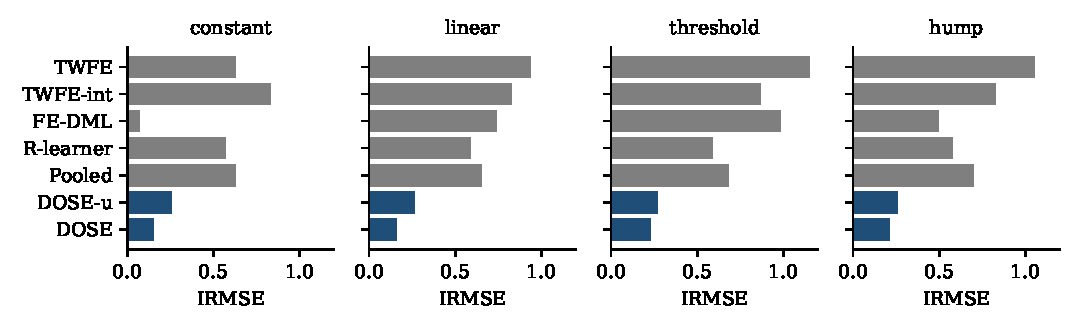
\includegraphics[width=\textwidth]{figures/sim_irmse.pdf}
\caption{IRMSE of the estimated effect function by design (stylised design, 100 replications). DOSE denotes Panel-DOSE and DOSE-u its unpenalised version; green bars are ablations; Oracle is the infeasible latent-information benchmark.}\label{fig:simirmse}
\end{figure}

\begin{figure}[!t]
\centering
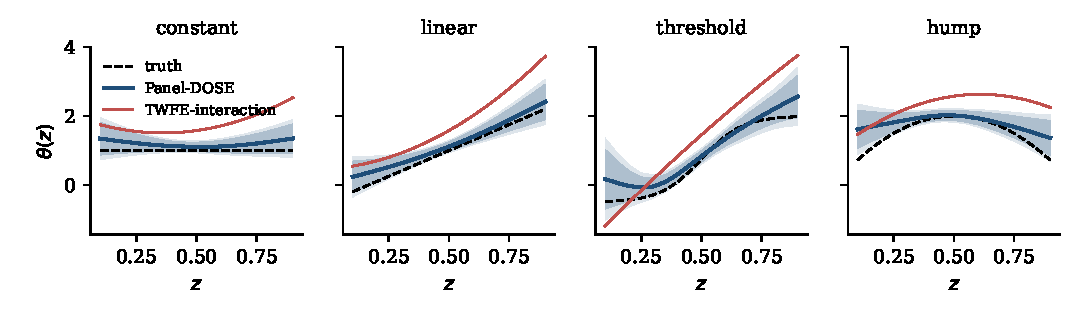
\includegraphics[width=\textwidth]{figures/sim_curves.pdf}
\caption{One simulated sample per design. Dashed black: true $\theta(z)$; blue: Panel-DOSE with 95\% pointwise (dark) and simultaneous (light) bands; red: TWFE with quadratic interaction.}\label{fig:simcurves}
\end{figure}

\begin{table}[!t]
\centering
\begin{threeparttable}
\caption{Stylised design, threshold $\theta$: sensitivity to sample size and confounding.}\label{tab:simsens}
\scriptsize
\setlength{\tabcolsep}{3pt}
\begin{tabular}{lcccccc}
\toprule
 & $G=50$ & $G=100$ & $G=100$ & $G=100$ & $G=100$ & $G=200$\\
 & $\rho=1$ & $\rho=0.25$ & $\rho=0.5$ & $\rho=1$ & $\rho=2$ & $\rho=1$\\
\midrule
%% BEGIN tables/sim_sens.tex (generated by code/make_outputs.py)
\multicolumn{7}{l}{\textit{IRMSE}}\\
\quad TWFE-interaction & 0.89 & 0.46 & 0.56 & 0.87 & 1.66 & 0.87\\
\quad TWFE-spline & 0.37 & 0.17 & 0.20 & 0.29 & 0.52 & 0.25\\
\quad FE-DML + R-learner (tuned) & 0.36 & 0.27 & 0.28 & 0.28 & 0.33 & 0.21\\
\quad Panel-DOSE (unpenalised) & 0.43 & 0.26 & 0.27 & 0.27 & 0.34 & 0.18\\
\quad Panel-DOSE & 0.34 & 0.22 & 0.22 & 0.23 & 0.29 & 0.14\\
\addlinespace\multicolumn{7}{l}{\textit{Pointwise coverage}}\\
\quad TWFE-interaction & 0.20 (0.01) & 0.25 (0.02) & 0.12 (0.01) & 0.16 (0.00) & 0.16 (0.01) & 0.11 (0.00)\\
\quad Panel-DOSE (unpenalised) & 0.92 (0.01) & 0.93 (0.01) & 0.92 (0.01) & 0.93 (0.01) & 0.91 (0.02) & 0.91 (0.01)\\
\quad Panel-DOSE & 0.86 (0.02) & 0.83 (0.02) & 0.82 (0.02) & 0.81 (0.02) & 0.75 (0.02) & 0.90 (0.01)\\
\addlinespace\multicolumn{7}{l}{\textit{Uniform coverage}}\\
\quad TWFE-interaction & 0.00 (0.00) & 0.00 (0.00) & 0.00 (0.00) & 0.00 (0.00) & 0.00 (0.00) & 0.00 (0.00)\\
\quad Panel-DOSE (unpenalised) & 0.82 (0.05) & 0.76 (0.06) & 0.76 (0.06) & 0.83 (0.04) & 0.84 (0.05) & 0.86 (0.05)\\
\quad Panel-DOSE & 0.62 (0.07) & 0.54 (0.07) & 0.58 (0.07) & 0.58 (0.05) & 0.42 (0.07) & 0.72 (0.06)\\
\addlinespace\multicolumn{7}{l}{\textit{Coverage of high--low contrast}}\\
\quad TWFE-interaction & 0.22 (0.06) & 0.22 (0.06) & 0.10 (0.04) & 0.03 (0.02) & 0.04 (0.03) & 0.00 (0.00)\\
\quad Panel-DOSE (unpenalised) & 0.94 (0.03) & 0.92 (0.04) & 0.96 (0.03) & 0.96 (0.02) & 1.00 (0.00) & 0.94 (0.03)\\
\quad Panel-DOSE & 0.96 (0.03) & 0.92 (0.04) & 0.88 (0.05) & 0.91 (0.03) & 0.94 (0.03) & 0.92 (0.04)\\
%% END tables/sim_sens
\bottomrule
\end{tabular}
\begin{tablenotes}\scriptsize
\item Notes: 50 replications per cell except $G=100$, $\rho=1$ (100). Monte Carlo standard errors of coverage rates in parentheses. $\rho$ scales the nonlinear confounding in the outcome equation.
\end{tablenotes}
\end{threeparttable}
\end{table}

\subsection{Plasmode design}\label{sec:plasmode}

The stylised design has less noise and more residual variation in adoption than the application. The plasmode design \citep{franklin2014plasmode} keeps the actual controls, treatment, moderators and panel structure of the baseline sample of Section~\ref{sec:emp} ($\nm{nobs}$ observations, $\nm{ncty}$ countries) and regenerates only the outcome, as $Y^*_{it}=\theta(Z_{it})D_{it}+\hat g(F_{it})+w_i\hat e_{it}$. Here $\hat g$ is a boosted-tree fit of observed productivity growth on the nuisance features, $\hat e_{it}$ are the corresponding residuals, and $w_i$ are Rademacher weights drawn per country. The errors thus keep their size, heteroskedasticity and within-country dependence, while any association with $D$ is randomised away. The design inherits the limitations of a single pilot fit: $\hat g$ is smoother than the true control function and the design holds the panel fixed. For each of the three moderators we consider no effect (the size of the constancy test), a linear gradient (the size of the linearity test and the power of the constancy test) and a smooth threshold (curvature). The linear and threshold functions are scaled so that their tercile contrast equals the minimum detectable contrast of the application, 2.8 times the baseline standard error ($\nm{ptargetA}$, $\nm{ptargetB}$ and $\nm{ptargetC}$). The estimator is run exactly as in the application, with five repetitions of the split and a cross-validated penalty. We use $\nm{prepsnA}$ replications under no effect, so that the Monte Carlo standard error of a rejection rate of 5\% is $\nm{pmcseA}$ percentage points, and $\nm{prepslA}$ under each alternative.

Table~\ref{tab:plasmode} reports the results. Under no effect, the penalised constancy test rejects in $\nm{prcnA}$ and $\nm{prcnB}$ of the replications for schooling and initial productivity, close to the nominal 5\% given a Monte Carlo standard error of about $\nm{pmcseA}$ percentage points, and the unpenalised test in $\nm{prcnuA}$ and $\nm{prcnuB}$. For years since take-off, however, both tests are clearly over-sized ($\nm{prcnC}$ penalised, $\nm{prcnuC}$ unpenalised): this moderator is very skewed, its lowest values come from a few late adopters, and the curve is poorly determined there. We therefore do not use the constancy test for this moderator to claim heterogeneity, and a non-rejection for it is a fortiori uninformative about its absence. Under the linear gradient, the penalised linearity test rejects in $\nm{prllA}$, $\nm{prllB}$ and $\nm{prllC}$ of the replications, and the constancy test has power $\nm{prclA}$, $\nm{prclB}$ and $\nm{prclC}$ against a gradient of the size of the minimum detectable contrast. The contrast intervals cover the true contrast in $\nm{pcovnA}$--$\nm{pcovnB}$ of replications under no effect for schooling and initial productivity and in $\nm{pcovnC}$ for years since take-off; the contrast estimates are biased by $\nm{pbiasnA}$, $\nm{pbiasnB}$ and $\nm{pbiasnC}$ under no effect. Under curvature, the bands under-cover: simultaneous bands for the penalised fit cover the threshold function in $\nm{psimtB}$ of the replications for initial productivity, which reflects the smoothing bias described in Remark~\ref{rem:scope}. The linear TWFE benchmarks are much less reliable along initial productivity (Table~\ref{tab:plasmodetwfe} in \ref{app:tables}): with no effect at all, the linear-interaction and spline-control contrasts are biased by $\nm{ptwibiasB}$ and $\nm{ptwsbiasB}$ and reject in $\nm{ptwirejB}$ and $\nm{ptwsrejB}$ of the replications.

\begin{table}[!t]
\centering
\begin{threeparttable}
\caption{Plasmode design built on the empirical panel: Panel-DOSE.}\label{tab:plasmode}
\scriptsize
\setlength{\tabcolsep}{2.5pt}
\begin{tabular}{lcccccccc}
\toprule
 & \multicolumn{4}{c}{High--low tercile contrast} & \multicolumn{2}{c}{Test rejection} & \multicolumn{2}{c}{Band coverage}\\
\cmidrule(lr){2-5}\cmidrule(lr){6-7}\cmidrule(lr){8-9}
True $\theta$ & Bias & RMSE & Coverage & Rejection & Constancy & Linearity & Pointwise & Simultaneous\\
\midrule
%% BEGIN tables/plasmode.tex (generated by code/make_outputs.py)
\multicolumn{9}{l}{\textit{Moderator: Schooling}}\\
\quad no effect & -0.87 & 2.40 & 0.96 (0.01) & 0.04 (0.01) & 0.04 (0.01) & 0.03 (0.01) & 0.92 (0.01) & 0.95 (0.02)\\
\quad no effect, unpenalised & -0.99 & 2.24 & 0.97 (0.01) & 0.03 (0.01) & 0.03 (0.01) & 0.03 (0.01) & 0.95 (0.01) & 0.95 (0.01)\\
\quad linear gradient & 0.52 & 2.19 & 0.99 (0.01) & 0.93 (0.03) & 0.92 (0.03) & 0.01 (0.01) & 0.91 (0.02) & 0.88 (0.03)\\
\quad linear gradient, unpenalised & 0.21 & 1.90 & 1.00 (0.00) & 0.96 (0.02) & 0.85 (0.04) & 0.03 (0.02) & 0.94 (0.01) & 0.95 (0.02)\\
\quad threshold & 0.93 & 2.04 & 1.00 (0.00) & 0.99 (0.01) & 0.99 (0.01) & 0.15 (0.04) & 0.91 (0.01) & 0.90 (0.03)\\
\quad threshold, unpenalised & -0.02 & 1.86 & 0.99 (0.01) & 0.96 (0.02) & 0.92 (0.03) & 0.12 (0.03) & 0.94 (0.01) & 0.98 (0.01)\\
\addlinespace
\multicolumn{9}{l}{\textit{Moderator: Initial productivity}}\\
\quad no effect & -1.11 & 2.34 & 0.94 (0.02) & 0.07 (0.02) & 0.06 (0.02) & 0.07 (0.02) & 0.91 (0.01) & 0.92 (0.02)\\
\quad no effect, unpenalised & -1.26 & 2.93 & 0.90 (0.02) & 0.10 (0.02) & 0.09 (0.02) & 0.12 (0.02) & 0.93 (0.01) & 0.90 (0.02)\\
\quad linear gradient & -0.57 & 2.29 & 0.98 (0.01) & 0.92 (0.03) & 0.87 (0.03) & 0.05 (0.02) & 0.91 (0.02) & 0.91 (0.03)\\
\quad linear gradient, unpenalised & -0.56 & 2.94 & 0.94 (0.02) & 0.69 (0.05) & 0.94 (0.02) & 0.18 (0.04) & 0.91 (0.01) & 0.87 (0.03)\\
\quad threshold & -1.13 & 2.34 & 0.96 (0.02) & 0.89 (0.03) & 0.87 (0.03) & 0.11 (0.03) & 0.85 (0.02) & 0.72 (0.05)\\
\quad threshold, unpenalised & -0.52 & 2.87 & 0.94 (0.02) & 0.75 (0.04) & 0.98 (0.01) & 0.26 (0.04) & 0.91 (0.01) & 0.87 (0.03)\\
\addlinespace
\multicolumn{9}{l}{\textit{Moderator: Years since take-off}}\\
\quad no effect & 3.87 & 6.60 & 0.94 (0.02) & 0.07 (0.02) & 0.21 (0.03) & 0.12 (0.02) & 0.90 (0.01) & 0.86 (0.02)\\
\quad no effect, unpenalised & 2.73 & 8.26 & 0.98 (0.01) & 0.01 (0.01) & 0.26 (0.03) & 0.17 (0.03) & 0.88 (0.01) & 0.80 (0.03)\\
\quad linear gradient & 1.56 & 4.45 & 1.00 (0.00) & 1.00 (0.00) & 1.00 (0.00) & 0.07 (0.03) & 0.94 (0.01) & 0.89 (0.03)\\
\quad linear gradient, unpenalised & -0.27 & 7.21 & 1.00 (0.00) & 0.90 (0.03) & 1.00 (0.00) & 0.08 (0.03) & 0.91 (0.01) & 0.89 (0.03)\\
\quad threshold & 3.25 & 6.38 & 0.99 (0.01) & 1.00 (0.00) & 1.00 (0.00) & 0.79 (0.04) & 0.93 (0.01) & 0.91 (0.03)\\
\quad threshold, unpenalised & -0.08 & 7.21 & 1.00 (0.00) & 0.88 (0.03) & 1.00 (0.00) & 0.73 (0.04) & 0.93 (0.01) & 0.92 (0.03)\\
%% END tables/plasmode
\bottomrule
\end{tabular}
\begin{tablenotes}\scriptsize
\item Notes: Monte Carlo standard errors in parentheses. Under no effect, ``Rejection'' is the size of the 5\% test that the contrast is zero and ``Constancy'' and ``Linearity'' are the sizes of the sup-$t$ tests; under a linear gradient, ``Linearity'' is a size and the other rejection rates are powers. Band coverage refers to the true $\theta$ on a 17-point grid between the 5th and 95th percentiles of the moderator.
\end{tablenotes}
\end{threeparttable}
\end{table}

%% ===========================================================================
\section{Empirical application: internet diffusion and productivity growth, 1996--2025}\label{sec:emp}

\subsection{Data and specification}

The main data set combines the World Bank's World Development Indicators (WDI, July 2026 release, retrieved in September 2026) with the UNDP Human Development Report 2025. The outcome is annual growth of GDP per person employed at constant 2021 PPP prices, $Y_{it}=100\,\Delta\ln(\text{GDP}_{it}/\text{EMP}_{it})$, which WDI compiles from national accounts and the modelled employment estimates of the International Labour Organization (ILO) and which is available up to 2025. The treatment is the share of the population using the internet (ITU) in year $t-1$, measured on $[0,1]$. It is a lagged \emph{level}, not a change: $\theta$ compares growth in years in which a country's internet share was higher with growth in years in which it was lower, conditional on the controls and on country and year effects, and one tenth of $\theta$ is the difference in growth (in pp) associated with a ten-percentage-point higher lagged share. In the baseline, the controls are lagged mean years of schooling, the lagged government consumption share, trade openness, population growth, the age-dependency ratio and the urban population share, and initial log GDP per worker, measured as the average over 1991--1995.

The baseline deliberately excludes three groups of variables used in the earlier literature. Lagged productivity levels and growth are excluded because they violate strict exogeneity mechanically (Section~\ref{sec:method}). Mobile and fixed-broadband subscriptions are excluded because they measure the same diffusion process, so that controlling for them turns the estimand into the association of internet use net of co-diffusing technologies. The investment share is excluded because it is a likely channel. We report specifications that add each group back. Variables that enter only such robustness checks do not restrict the baseline sample: an observation is used if the outcome, the treatment and the baseline controls are observed. The sample covers 1996--2025, drops growth observations below the 1st and above the 99th percentile, and keeps countries with at least 15 usable years. Table~\ref{tab:flow} in \ref{app:data} shows the observations lost at each step. We screen the adoption series for implausible values and jumps; the rules flag $\nm{nflags}$ values, for example a rise in Fiji's mobile subscriptions from 361 to 574 per 100 people in one year (\ref{app:data}). Flagged values are set to missing, so flags in the mobile and broadband series affect only the specifications that use these series. The resulting panel contains $\nm{nobs}$ observations on $\nm{ncty}$ countries. It includes $\nm{covhi}$ of $\nm{tothi}$ high-income, $\nm{covum}$ of $\nm{totum}$ upper-middle-income, $\nm{covlm}$ of $\nm{totlm}$ lower-middle-income and $\nm{covli}$ of $\nm{totli}$ low-income economies. Economies are excluded mainly because productivity, schooling or government-consumption data are missing; many of the excluded low-income economies are fragile or conflict-affected states (e.g.\ Afghanistan, Somalia, South Sudan, Yemen). An earlier version of this paper also required the other ICT series, the investment share, lagged productivity and a second lag of the treatment to be observed; that common sample ($\nm{nobscommon}$ observations, $\nm{nctycommon}$ countries) is reported as a robustness check. Table~\ref{tab:desc} reports descriptive statistics.

We also use two releases of the Penn World Table \citep{feenstra2015pwt}: version 11.0 \citep{pwt11}, which covers $\nm{nctypwtel}$ countries over 1996--2023 in our sample ($\nm{npwtel}$ observations), and version 10.0, which ends in 2019 ($\nm{nctypwtten}$ countries, $\nm{npwtten}$ observations). The outcome is growth of real GDP at constant national prices per person engaged (\texttt{rgdpna}/\texttt{emp}), the variable PWT recommends for growth comparisons. The initial-productivity moderator is instead output-side real GDP at current PPPs per person engaged (\texttt{cgdpo}/\texttt{emp}), averaged over 1991--1995, which PWT recommends for comparing productive capacity across countries at a point in time; we report the national-prices level as a sensitivity check. PWT 10.0 expresses levels in 2017 and PWT 11.0 in 2021 US dollars. Because the knots and terciles are placed at quantiles and the B-spline basis is invariant to affine transformations of the moderator, a change of base year does not by itself affect the estimates; what matters is how the releases rank countries. The PWT panels use the PWT human-capital index and the same controls as the WDI baseline plus the labour share; PWT also provides total factor productivity (TFP).

We estimate model~\eqref{eq:model} with three moderators corresponding to the predictions of Section~\ref{sec:pred}: mean years of schooling (absorptive capacity), initial log GDP per worker (distance to the frontier and leapfrogging) and years since the internet-user share first reached 10\% (the J-curve). Using initial rather than lagged productivity as the development moderator avoids the mechanical link with the outcome and sorts countries rather than country-years into terciles. Years since take-off is computed from the whole adoption path, so before take-off its (negative) value uses the future year in which the share crosses 10\%; it describes the stage of the diffusion life cycle but is not predetermined. We therefore also use a predetermined version that is zero until take-off and counts the years since take-off afterwards. Panel-DOSE uses LightGBM with 400 trees, five country-level folds, five repetitions of the split and cubic B-splines with four interior knots; standard errors are clustered by country. Robustness checks use three repetitions of the split to save computation, so their FE-DML estimates can differ slightly from the baseline even when the specification is otherwise the same.

Figure~\ref{fig:desc} shows the variation that identifies the estimates. Internet use diffused everywhere, but at different times. In the countries with the highest initial productivity, about half of the population was online by the mid-2000s, whereas in the least productive third the share passed one fifth only in the mid-2010s and one half at the end of the sample. Smoothed productivity growth was highest in the low and middle groups during the 2000s and fell around 2009 and 2020. Year effects absorb these common shocks, so the estimates rely on differences across countries in the timing of adoption relative to their own productivity paths.

\begin{figure}[!t]
\centering
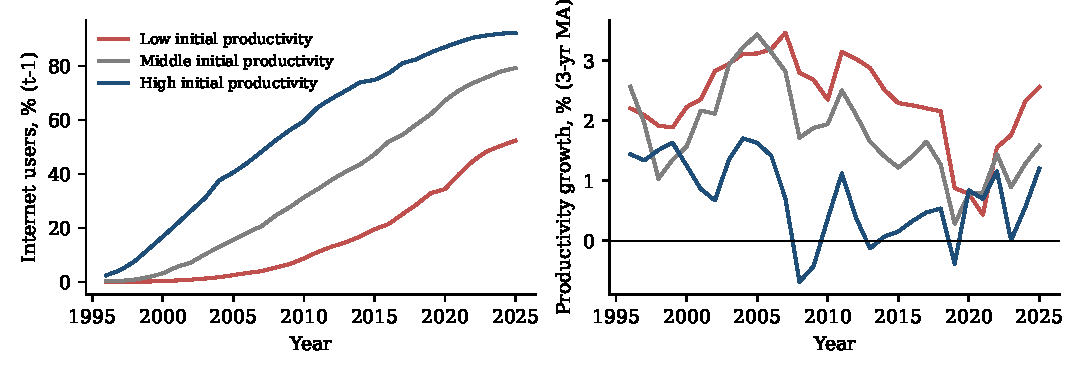
\includegraphics[width=\textwidth]{figures/desc_diffusion.pdf}
\caption{Internet diffusion and labour-productivity growth by tercile of initial GDP per worker, 1996--2025: (left) sample average of the lagged internet-user share by year; (right) centred three-year moving average of the yearly sample averages of productivity growth.}\label{fig:desc}
\end{figure}

\begin{table}[!t]
\centering
\begin{threeparttable}
\caption{Descriptive statistics, baseline sample, 1996--2025.}\label{tab:desc}
\small
\begin{tabular}{lccccc}
\toprule
Variable & Obs. & Mean & Std.\ dev. & Min & Max\\
\midrule
%% BEGIN tables/descriptives.tex (generated by code/make_outputs.py)
Labour-productivity growth (\%) & 4075 & 1.622 & 3.458 & -10.758 & 12.459\\
Internet users, share ($t-1$) & 4075 & 0.367 & 0.333 & 0.000 & 1.000\\
Mobile subscriptions per capita ($t-1$) & 4030 & 0.751 & 0.523 & 0.000 & 2.471\\
Fixed broadband per capita ($t-1$) & 3995 & 0.091 & 0.128 & 0.000 & 0.489\\
Mean years of schooling ($t-1$) & 4075 & 8.480 & 3.270 & 0.975 & 14.325\\
Initial log GDP per worker (pre-sample) & 4075 & 10.157 & 1.106 & 7.097 & 12.470\\
Investment share ($t-1$) & 4047 & 0.240 & 0.073 & -0.024 & 0.713\\
Government consumption share ($t-1$) & 4075 & 0.161 & 0.070 & 0.020 & 1.477\\
Trade openness ($t-1$) & 4075 & 0.855 & 0.534 & 0.156 & 4.426\\
Population growth, \% ($t-1$) & 4075 & 1.347 & 1.506 & -10.927 & 21.700\\
Age-dependency ratio ($t-1$) & 4075 & 0.604 & 0.177 & 0.173 & 1.140\\
Urban population share ($t-1$) & 4075 & 0.605 & 0.215 & 0.103 & 1.000\\
Years since internet take-off ($t-1$) & 4075 & 4.070 & 10.493 & -26.000 & 29.000\\
GDP per capita growth (\%) & 4075 & 2.107 & 3.686 & -21.001 & 16.071\\
%% END tables/descriptives
\bottomrule
\end{tabular}
\begin{tablenotes}\footnotesize
\item Sources: World Development Indicators (World Bank, July 2026 release), including ITU adoption series; UNDP Human Development Report 2025 (mean years of schooling). Years since take-off is negative before the internet-user share first reaches 10\%.
\end{tablenotes}
\end{threeparttable}
\end{table}

\subsection{The average association}

In the baseline, the headline FE-DML estimate is $\nm{fedml}$ (s.e.\ $\nm{fedmlse}$): a ten-percentage-point higher lagged internet-user share is associated with $\nm{fedmlten}$ pp lower productivity growth, with a country-clustered 95\% interval of $[\nm{cilo},\nm{cihi}]$ pp. Two-way clustering by country and year gives a standard error of $\nm{twse}$ and an interval of $[\nm{cilotw},\nm{cihitw}]$ pp; with about 30 years, this interval should itself be read with caution. The TWFE estimate with the same controls is $\nm{twfe}$ ($\nm{twfese}$), and the equally weighted sample-average effect from the sieve is $\nm{savg}$ ($\nm{savgse}$). Over the average within-country range of the internet-user share in the sample ($\nm{rise}$ points), the headline estimate corresponds to $\nm{riseimpl}$ pp lower annual growth; the upper end of the baseline interval corresponds to $\nm{riseimplhi}$ pp. These bounds are specific to the baseline specification and its assumptions; other specifications give wider intervals that include zero.

The FE-DML estimate is negative in every specification we estimate (Table~\ref{tab:emp} and \ref{app:tables}), but its magnitude and precision vary. The estimate is $\nm{rf}$ ($\nm{rfse}$) with random-forest nuisance functions, $\nm{ry}$ ($\nm{ryse}$) with region-by-year effects, $\nm{precovid}$ ($\nm{precovidse}$) before COVID-19, $\nm{nocovid}$ ($\nm{nocovidse}$) without 2020--2021, $\nm{gdppc}$ ($\nm{gdppcse}$) with GDP-per-capita growth as the outcome, $\nm{spi}$ ($\nm{spise}$) in countries with above-median statistical capacity (World Bank Statistical Performance Indicators, SPI), $\nm{pwtel}$ ($\nm{pwtelse}$) in PWT 11.0 and $\nm{pwtten}$ ($\nm{pwttense}$) in PWT 10.0. In the common sample of the earlier version it is $\nm{common}$ ($\nm{commonse}$). Adding mobile and broadband subscriptions to the controls reduces it to $\nm{mobbb}$ ($\nm{mobbbse}$), and the original specification with lagged productivity, lagged growth, investment and the other ICT measures gives $\nm{orig}$ ($\nm{origse}$). These specifications estimate a different quantity---the association of internet use net of co-diffusing technologies---and the fall in the estimate shows how much of the baseline association the three adoption series share. A composite ICT index as the treatment gives $\nm{ict}$ ($\nm{ictse}$) per unit of the index. Excluding resource exporters gives $\nm{nores}$ ($\nm{noresse}$). Weighting the average of $\theta(Z)$ by population, which gives China and India large weights, gives $\nm{popwavg}$ ($\nm{popwavgse}$) in the schooling specification.

The residual variation that identifies the estimates is limited. After the nuisance step and the within transformation, $\nm{idvar}$ of the within-country variance of adoption remains ($\nm{idvartot}$\% of its total variance), and only $\nm{idvarlowA}$--$\nm{idvarlowB}$ in the lowest tercile of schooling or initial productivity, where the median adoption share is $\nm{dmedlowA}$--$\nm{dmedlowB}$. Estimates for the least developed economies are therefore imprecise.

\paragraph{Exogeneity and dynamics}
Strict exogeneity implies that future adoption should not predict current growth once current adoption is controlled for \citep[Section 10.7]{wooldridge2010}. Adding the lead $D_{i,t+1}$ to the baseline gives a lead coefficient of $\nm{leadtw}$ ($\nm{leadtwse}$) with TWFE and $\nm{leaddml}$ ($\nm{leaddmlse}$) with FE-DML (Table~\ref{tab:dyn}). Neither is significant, but both are imprecise, so the test has little power against moderate feedback from growth to adoption. Table~\ref{tab:dyn} and Figure~\ref{fig:dyn}(b) report local projections \citep{jorda2005lp} of the cumulative change in log productivity from $t-1$ to $t+h$ on the internet share in $t-1$, with the baseline controls; horizon $h$ covers $h+1$ years of growth. The cumulative association becomes more negative with the horizon: $\nm{lpb}$ pp per ten points over two years ($h=1$), $\nm{lpd}$ pp over four years and $\nm{lpi}$ pp over nine years, with widening intervals. Because longer horizons lose the last years of the sample, we also estimate every horizon on the $\nm{lpcn}$ observations for which the nine-year change is observed; the pattern is the same (from $\nm{lpca}$ pp at $h=0$ to $\nm{lpci}$ pp at $h=8$). These regressions of cumulative growth on a persistent adoption level with static controls describe how the conditional association evolves; they do not identify an impulse response to an adoption shock. Within the horizons we observe, they show no delayed positive association that offsets the short-run one. Non-overlapping five-year averages \citep{islam1995growth} give $\nm{fytwfe}$ ($\nm{fytwfese}$) with TWFE and $\nm{fyfedml}$ ($\nm{fyfedmlse}$) with FE-DML.

The picture is different across countries. We regress average annual productivity growth over 2000--2024, i.e.\ $100(\ln\mathrm{LP}_{2024}-\ln\mathrm{LP}_{1999})/25$, which is the mean of the annual growth rates used in the panel, on the change in the panel treatment over the same years, $D_{2024}-D_{2000}$ (the internet share of 2023 minus that of 1999), with the controls of 2000 (mostly 1999 values). Economies whose internet share rose more grew faster, by about $\nm{ldolsten}$ pp per year per ten points (OLS $\nm{ldols}$, s.e.\ $\nm{ldolsse}$; DML $\nm{lddml}$, s.e.\ $\nm{lddmlse}$; $\nm{ldn}$ countries). Because this comparison does not remove country effects, it is consistent with faster-growing economies adopting faster rather than with adoption raising growth. An instrumental-variable check that instruments adoption with the 1990 density of fixed telephone lines interacted with the global diffusion curve has a weak first stage ($F=\nm{ivf}$) and gives an imprecise two-stage least squares (2SLS) estimate of $\nm{iv}$ ($\nm{ivse}$); we report it for completeness only.

\paragraph{Comparison with broadband studies}
Our main estimate concerns internet users, per-worker growth and a global panel, whereas \citet{czernich2011broadband} study broadband, per-capita growth and OECD countries over 1996--2007 with an instrumental-variable design. As a descriptive benchmark closer to their setting, we use fixed broadband subscriptions as the treatment and GDP-per-capita growth as the outcome in high-income economies. The FE-DML estimate is $\nm{cz}$ ($\nm{czse}$), i.e.\ $[\nm{czlo},\nm{czhi}]$ pp per ten points. Because the populations, periods, treatments and estimands differ, and ours rests on selection on observables, this comparison cannot establish whether the two sets of results are compatible; it shows only that a conditional association of the size they report is not visible in these data.

\begin{table}[!t]
\centering
\begin{threeparttable}
\caption{Dynamic specifications and alternative designs.}\label{tab:dyn}
\scriptsize
\setlength{\tabcolsep}{3pt}
\begin{tabular}{lccccccc}
\toprule
\multicolumn{8}{l}{\textit{Panel A. Local projections: change in log productivity ($\times100$) from $t-1$ to $t+h$}}\\
 & \multicolumn{3}{c}{All available observations} & \multicolumn{2}{c}{Common sample} & \multicolumn{2}{c}{High $-$ low}\\
\cmidrule(lr){2-4}\cmidrule(lr){5-6}\cmidrule(lr){7-8}
Horizon (years) & Average & (s.e.) & Obs. & Average & (s.e.) & Contrast & (s.e.)\\
\midrule
%% BEGIN tables/emp_lp.tex (generated by code/make_outputs.py)
$h=0$ (1) & $-2.92^{**}$ & (1.35) & 4,075 & $-4.46^{***}$ & (1.54) & $-0.25$ & (3.06)\\
$h=1$ (2) & $-5.25^{**}$ & (2.62) & 3,933 & $-9.29^{***}$ & (2.95) & $-0.42$ & (5.79)\\
$h=2$ (3) & $-9.03^{**}$ & (3.60) & 3,792 & $-11.23^{**}$ & (4.50) & $0.70$ & (8.53)\\
$h=3$ (4) & $-9.06^{*}$ & (4.83) & 3,649 & $-13.77^{**}$ & (5.78) & $3.86$ & (13.53)\\
$h=4$ (5) & $-11.71^{*}$ & (6.91) & 3,508 & $-14.12^{*}$ & (7.27) & $14.16$ & (18.63)\\
$h=5$ (6) & $-10.48$ & (7.91) & 3,370 & $-14.76^{*}$ & (8.57) & $25.94$ & (21.85)\\
$h=6$ (7) & $-11.72$ & (8.49) & 3,230 & $-16.32^{*}$ & (9.51) & $41.42$ & (26.16)\\
$h=7$ (8) & $-14.70$ & (9.75) & 3,087 & $-15.73$ & (10.35) & $39.80$ & (30.76)\\
$h=8$ (9) & $-19.77^{*}$ & (11.17) & 2,941 & $-19.77^{*}$ & (11.17) & $59.02^{*}$ & (35.29)\\
%% END tables/emp_lp
\midrule
\multicolumn{8}{l}{\textit{Panel B. Alternative designs}}\\
Specification & Estimate & (s.e.) & Obs. & & & & \\
\midrule
%% BEGIN tables/emp_dyn.tex (generated by code/make_outputs.py)
Five-year averages, TWFE & $-2.43^{***}$ & (0.84) & 834 \\
Five-year averages, FE-DML & $-2.54^{*}$ & (1.39) & 834 \\
Long difference, OLS & $2.21^{***}$ & (0.62) & 117 \\
Long difference, DML & $2.17^{*}$ & (1.14) & 117 \\
Lead $D_{t+1}$, TWFE & $-0.87$ & (1.85) & 3,923 \\
Lead $D_{t+1}$, FE-DML & $-1.27$ & (2.03) & 3,923 \\
Fixed-line IV (2SLS), first-stage $F=5.6$ & $-3.78$ & (4.00) & 3,977 \\
Broadband, GDP p.c. growth, high income & $-2.32$ & (2.44) & 1,545 \\
Broadband, GDP p.c. growth, all countries & $-7.34^{***}$ & (2.34) & 3,995 \\
%% END tables/emp_dyn
\bottomrule
\end{tabular}
\begin{tablenotes}\footnotesize
\item Notes: coefficients per unit of adoption (0--1); divide by 10 for a ten-point difference. Panel A: FE-DML average and Panel-DOSE tercile contrast by initial log GDP per worker, baseline controls, three repetitions of the split (so the $h=0$ average differs slightly from the five-split baseline); the horizon in parentheses is the number of annual growth rates covered, $h+1$. ``Common sample'': observations for which the nine-year change is observed. Five-year averages: non-overlapping periods 1996--2000 to 2021--2025, treatment and controls at the start of the period. Long difference: average annual growth of GDP per worker over 2000--2024 on $D_{2024}-D_{2000}$ (internet share 2023 minus 1999), with 2000 values of the controls; OLS with HC1 standard errors and cross-fitted partially linear DML. Lead: coefficient on $D_{t+1}$ when it is added to the baseline (strict-exogeneity check). IV: 2SLS with country and year effects; instrument = 1990 fixed-line density $\times$ leave-one-out global internet share. Broadband rows: FE-DML with fixed broadband subscriptions as treatment and GDP-per-capita growth as outcome. $^{*}$, $^{**}$, $^{***}$: 10\%, 5\%, 1\%.
\end{tablenotes}
\end{threeparttable}
\end{table}

\subsection{Heterogeneity}

Table~\ref{tab:emp} and Figure~\ref{fig:emp} report the heterogeneity estimates. Table~\ref{tab:diag} in \ref{app:tables} reports the selected penalties, effective degrees of freedom, identifying variation and treatment support by tercile. The bands in Figure~\ref{fig:emp} describe the penalised fit (Remark~\ref{rem:scope}); the tests of heterogeneity are the constancy tests.

\paragraph{Schooling}
The association does not vary with schooling. The estimated function is nearly flat (Figure~\ref{fig:emp}a), the high-minus-low tercile contrast is $\nm{diffA}$ (s.e.\ $\nm{diffseA}$), the BLP slope is $\nm{blpA}$ ($\nm{blpseA}$) per year of schooling, and the constancy test does not reject ($p=\nm{pconstA}$). The absorptive-capacity prediction of a positive gradient is therefore not supported, but the data cannot rule out moderate gradients either: the 95\% interval for the contrast is $[\nm{ciloA},\nm{cihiA}]$ pp per ten points, and the minimum detectable contrast (80\% power at 5\%) is about $\nm{mdeA}$ pp per ten points. A null result for heterogeneity is not evidence against complementarities of this size. The sign of the contrast varies across robustness checks; in the common sample of the earlier version it is $\nm{commondiffA}$ ($\nm{commondiffseA}$). Learning-adjusted years of schooling, which account for the quality of schooling \citep{angrist2021learning}, give a similar picture (contrast $\nm{laysdiff}$, s.e.\ $\nm{laysdiffse}$).

\paragraph{Initial productivity}
Along initial productivity, the WDI estimates show no monotone gradient. The contrast is $\nm{diffB}$ ($\nm{diffseB}$) and the constancy test gives $p=\nm{pconstB}$. The estimated function dips in the middle of the distribution (Figure~\ref{fig:emp}b), and in several checks the constancy test rejects at 5\%: without the penalty ($p=\nm{pconstuB}$), with region-by-year effects ($p=\nm{rypB}$) and in a few others in \ref{app:tables}. All of these fits select a small penalty and use five to eight effective degrees of freedom; the unpenalised test is somewhat over-sized for this moderator in the plasmode ($\nm{prcnuB}$ at the 5\% level, Section~\ref{sec:plasmode}), and the tercile contrasts of these checks have different signs. We read them as weak evidence of non-monotone variation, not as support for the monotone gradient that the leapfrogging or frontier arguments predict. Excluding the bottom 5\% of the moderator gives a contrast of $\nm{diffx5B}$ ($\nm{diffx5seB}$), and using only countries with pre-sample productivity data gives $\nm{presmpdiff}$ ($\nm{presmpdiffse}$). Distance to the US frontier as the moderator, with terciles formed within year, gives $\nm{distusdiff}$ ($\nm{distusdiffse}$). The linear benchmarks find a positive gradient: $\nm{twgl}$ ($\nm{twglse}$) with a linear interaction and $\nm{twgs}$ ($\nm{twgsse}$) with spline controls. These values are close to the biases of the same estimators in the plasmode design without any effect ($\nm{ptwibiasB}$ and $\nm{ptwsbiasB}$), so they are what restrictive control functions produce in these data rather than evidence of a gradient.

\paragraph{Years since take-off}
The J-curve prediction receives no statistical support, and the constancy test for this moderator is over-sized in the plasmode, so even a rejection would have been weak evidence. In the baseline, the contrast between the last and the first tercile of time since take-off is $\nm{diffC}$ ($\nm{diffseC}$) and the constancy test does not reject ($p=\nm{pconstC}$); the first tercile contains the years long before take-off in countries that adopted late, where the estimate is very imprecise. With the predetermined moderator, which is zero before take-off, the contrast is $\nm{yprediff}$ ($\nm{yprediffse}$, $p=\nm{yprep}$), and in the common sample of the earlier version it is $\nm{commondiffC}$ ($\nm{commondiffseC}$). The earlier version's suggestion of a more negative association in the first years after take-off is therefore not robust to the choice of sample.

\paragraph{Dose response}
The marginal association $\hat f'(d)$ is negative over the range of adoption, most clearly at low adoption (Figure~\ref{fig:dyn}a), and linearity of $f$ is not rejected ($p=\nm{pdose}$). We do not detect departures from a linear conditional dose response over the evaluated support, so neither network effects nor saturation are visible in these data.

\paragraph{Multiple testing}
The three primary constancy tests give $p=\nm{pconstA}$, $\nm{pconstB}$ and $\nm{pconstC}$, with Holm-adjusted $p$-values of $\nm{holmA}$, $\nm{holmB}$ and $\nm{holmC}$. Without the penalty, the tests give $p=\nm{pconstuA}$, $\nm{pconstuB}$ and $\nm{pconstuC}$ (Holm $\nm{holmuA}$, $\nm{holmuB}$, $\nm{holmuC}$); the unpenalised tests are over-sized in the plasmode for the second and third moderators.

\begin{table}[!p]
\centering
\begin{threeparttable}
\caption{Heterogeneous associations of internet diffusion with labour-productivity growth.}\label{tab:emp}
\scriptsize
\setlength{\tabcolsep}{2.5pt}
\begin{tabular}{lccccccc}
\toprule
 & Average & \multicolumn{3}{c}{Tercile of moderator} & High $-$ & BLP & Constancy\\
\cmidrule(lr){3-5}
Specification & (FE-DML) & Low & Middle & High & low & slope & test $p$\\
\midrule
%% BEGIN tables/emp_main.tex (generated by code/make_outputs.py)
\multicolumn{8}{l}{\textit{Panel A. Moderator: mean years of schooling}}\\
\quad Baseline & $-2.79^{**}$ & $-1.99$ & $-2.92^{**}$ & $-3.07^{*}$ & $-0.67$ & $-0.19$ & 0.99\\
 & (1.30) & (2.80) & (1.45) & (1.70) & (3.30) & (0.45) & \\
\quad Common sample of the earlier version & $-2.53^{*}$ & $0.52$ & $-2.25^{*}$ & $-3.13^{*}$ & $-4.64$ & $-0.63$ & 0.38\\
 & (1.35) & (2.59) & (1.30) & (1.67) & (3.47) & (0.48) & \\
\quad Adding mobile and broadband & $-0.17$ & $-1.51$ & $-0.58$ & $0.47$ & $1.49$ & $0.20$ & 0.78\\
 & (1.20) & (2.47) & (1.24) & (1.59) & (2.94) & (0.40) & \\
\quad Random forest nuisance$^{\dagger}$ & $-2.89^{**}$ & $-2.67$ & $-3.24^{**}$ & $-2.87^{*}$ & $0.23$ & $0.00$ & 1.00\\
 & (1.17) & (2.17) & (1.28) & (1.48) & (2.82) & (0.38) & \\
\quad Region-by-year effects$^{\dagger}$ & $-2.58^{*}$ & $-1.68$ & $-2.51^{*}$ & $-3.03^{*}$ & $-1.43$ & $-0.19$ & 1.00\\
 & (1.35) & (3.06) & (1.47) & (1.57) & (3.46) & (0.48) & \\
\quad Pre-COVID sample, 1996--2019$^{\dagger}$ & $-3.51^{**}$ & $-2.32$ & $-3.39^{**}$ & $-3.70^{**}$ & $-1.30$ & $-0.18$ & 0.87\\
 & (1.48) & (3.38) & (1.61) & (1.86) & (4.18) & (0.57) & \\
\quad PWT 11.0, 1996--2023$^{\dagger}$ & $-3.27^{**}$ & $-13.35^{**}$ & $-2.29$ & $-1.24$ & $12.11^{*}$ & $9.84^{*}$ & 0.25\\
 & (1.30) & (6.23) & (1.83) & (1.28) & (6.89) & (5.46) & \\
\quad PWT 10.0, 1996--2019$^{\dagger}$ & $-1.42$ & $-7.15$ & $-0.60$ & $-2.33^{**}$ & $4.82$ & $6.76$ & 0.11\\
 & (1.66) & (5.70) & (2.07) & (1.09) & (5.89) & (4.60) & \\
\addlinespace
\multicolumn{8}{l}{\textit{Panel B. Moderator: initial log GDP per worker}}\\
\quad Baseline & $-2.79^{**}$ & $-1.00$ & $-5.29^{***}$ & $-1.15$ & $-0.25$ & $-0.47$ & 0.18\\
 & (1.30) & (2.80) & (1.80) & (1.43) & (3.13) & (1.25) & \\
\quad Common sample of the earlier version & $-2.53^{*}$ & $-1.46$ & $-2.55^{*}$ & $-3.19^{**}$ & $-1.01$ & $-0.56$ & 0.74\\
 & (1.35) & (2.72) & (1.37) & (1.38) & (3.21) & (1.25) & \\
\quad Adding mobile and broadband & $-0.17$ & $-0.66$ & $-0.57$ & $0.09$ & $0.77$ & $0.06$ & 1.00\\
 & (1.20) & (2.33) & (1.33) & (1.43) & (2.77) & (1.19) & \\
\quad Random forest nuisance$^{\dagger}$ & $-2.89^{**}$ & $-2.75$ & $-4.83^{***}$ & $-1.57$ & $0.75$ & $0.20$ & 0.51\\
 & (1.17) & (2.38) & (1.62) & (1.69) & (2.66) & (1.09) & \\
\quad Region-by-year effects$^{\dagger}$ & $-2.58^{*}$ & $-4.41$ & $-6.23^{***}$ & $0.53$ & $5.64$ & $2.97$ & 0.03\\
 & (1.35) & (3.83) & (2.06) & (1.64) & (3.74) & (1.86) & \\
\quad Pre-COVID sample, 1996--2019$^{\dagger}$ & $-3.51^{**}$ & $-0.75$ & $-5.28^{**}$ & $-1.64$ & $0.47$ & $-1.13$ & 0.59\\
 & (1.48) & (5.75) & (2.35) & (1.66) & (4.62) & (2.65) & \\
\quad WDI data, PWT 11.0 countries, 1996--2023$^{\dagger}$ & $-3.79^{***}$ & $-5.40^{**}$ & $-4.05^{***}$ & $-2.56$ & $2.12$ & $0.93$ & 0.61\\
 & (1.32) & (2.65) & (1.41) & (1.70) & (3.57) & (1.57) & \\
\quad PWT 11.0, 1996--2023$^{\dagger}$ & $-3.27^{**}$ & $-14.18^{***}$ & $-4.09^{***}$ & $1.42$ & $15.59^{***}$ & $8.30^{***}$ & $<$0.01\\
 & (1.30) & (3.49) & (1.57) & (1.30) & (4.06) & (2.37) & \\
\quad PWT 10.0, 1996--2019$^{\dagger}$ & $-1.42$ & $-12.20^{***}$ & $-3.10^{**}$ & $1.99$ & $14.19^{***}$ & $6.30^{***}$ & $<$0.01\\
 & (1.66) & (3.74) & (1.57) & (2.02) & (4.94) & (2.19) & \\
\addlinespace
\multicolumn{8}{l}{\textit{Panel C. Moderator: years since internet take-off (share $\geq$ 10\%)}}\\
\quad Baseline & $-2.15$ & $2.49$ & $-3.17^{**}$ & $-1.09$ & $-5.17$ & $-0.51$ & 0.36\\
 & (1.35) & (10.83) & (1.61) & (1.75) & (11.12) & (0.57) & \\
\quad Common sample of the earlier version & $-1.60$ & $-5.72$ & $-2.37$ & $-0.37$ & $5.35$ & $0.23$ & 0.68\\
 & (1.33) & (4.44) & (1.68) & (1.77) & (5.29) & (0.23) & \\
\quad Random forest nuisance$^{\dagger}$ & $-1.65$ & $8.67$ & $-3.02^{*}$ & $-0.79$ & $-9.71$ & $-0.86$ & 0.07\\
 & (1.39) & (14.02) & (1.65) & (1.74) & (14.11) & (0.75) & \\
\quad Region-by-year effects$^{\dagger}$ & $-1.65$ & $0.88$ & $-2.73^{*}$ & $-0.94$ & $-2.07$ & $-0.25$ & 0.29\\
 & (1.35) & (9.36) & (1.63) & (1.68) & (9.46) & (0.45) & \\
\quad Predetermined moderator (zero before take-off)$^{\dagger}$ & $-2.07$ & $-3.68^{*}$ & $-2.55^{*}$ & $-0.71$ & $2.97$ & $0.18$ & 0.47\\
 & (1.35) & (2.10) & (1.54) & (1.66) & (2.70) & (0.17) & \\
%% END tables/emp_main
\bottomrule
\end{tabular}
\begin{tablenotes}\scriptsize
\item Notes: Panel-DOSE estimates; standard errors clustered by country in parentheses. Coefficients are per unit of adoption (0--1); divide by 10 for a ten-point difference. The dependent variable is annual labour-productivity growth (\%) unless stated otherwise. Baseline: WDI panel ($\nm{ncty}$ countries, 1996--2025) with the controls listed in Section~\ref{sec:emp}. ``Common sample of the earlier version'': observations with every ICT series, the investment share, lagged productivity and the second lag of the treatment observed ($\nm{nctycommon}$ countries). ``Region-by-year effects'' replaces the year effects by World Bank region $\times$ year effects. PWT rows use the Penn World Table panels, with the PWT human-capital index (Panel A) and initial log PWT labour productivity at current PPPs (Panel B) as moderators. The BLP slope is per unit of the moderator (years of schooling, log points, years). ``Constancy test $p$'': sup-$t$ test that $\theta$ is constant. $^{\dagger}$: three repetitions of the sample split (five otherwise). The high-minus-low contrast is aggregated across splits as a functional in its own right, so it can differ slightly from the difference of the two tercile columns. $^{*}$, $^{**}$, $^{***}$: 10\%, 5\%, 1\%.
\end{tablenotes}
\end{threeparttable}
\end{table}

\begin{figure}[!t]
\centering
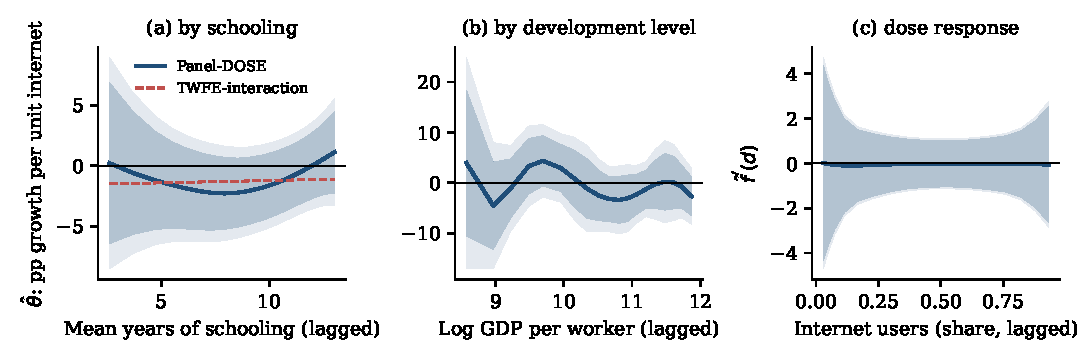
\includegraphics[width=\textwidth]{figures/emp_main.pdf}
\caption{Estimated association of lagged internet diffusion with labour-productivity growth, WDI panel 1996--2025: (a) by mean years of schooling and (b) by initial log GDP per worker, each with the TWFE linear-interaction estimate (dashed); (c) by years since the internet-user share first reached 10\%. Dark bands: 95\% pointwise; light bands: 95\% simultaneous, both for the penalised fit (Remark~\ref{rem:scope}). Grids span the 1st to 99th percentiles and the vertical axes show the full bands; tick marks show the distribution of the moderator.}\label{fig:emp}
\end{figure}

\begin{figure}[!t]
\centering
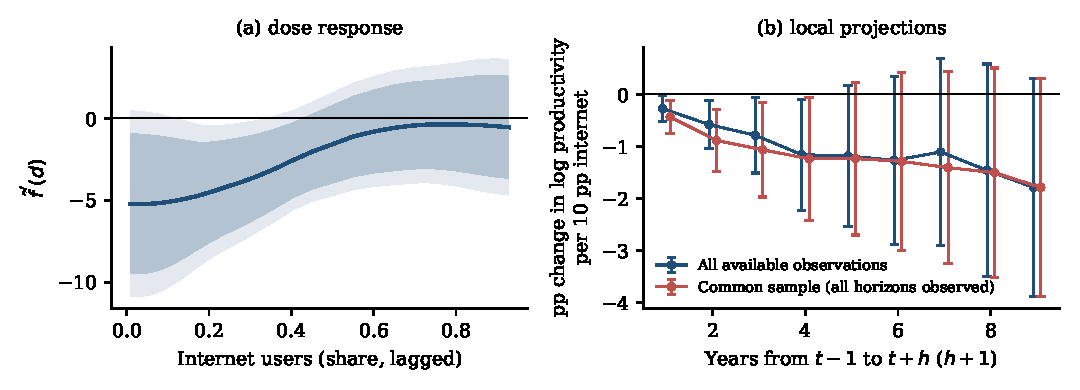
\includegraphics[width=\textwidth]{figures/emp_dyn.pdf}
\caption{(a) Marginal association $\hat f'(d)$ in the dose-response model, from the $\nm{dosestart}$th to the 95th percentile of adoption, with 95\% pointwise and simultaneous bands. (b) Local projections: change in log labour productivity ($\times100$) from $t-1$ to $t+h$ associated with a ten-point higher internet share in $t-1$, plotted against the number of years covered ($h+1$), for all available observations and for the common sample in which the nine-year change is observed, with 95\% intervals.}\label{fig:dyn}
\end{figure}

\subsection{Data sources and vintages}

The PWT panels tell a different story about heterogeneity (Panel B of Table~\ref{tab:emp} and Figure~\ref{fig:emprob}b). With the same specification, the contrast along initial productivity is $\nm{pwttenBdiff}$ ($\nm{pwttenBdiffse}$) in PWT 10.0 (1996--2019) and $\nm{pwtelBdiff}$ ($\nm{pwtelBdiffse}$) in PWT 11.0 (1996--2023), and the constancy test rejects in both ($p=\nm{pwttenBp}$ and $\nm{pwtelBp}$), against $\nm{wdipwtBdiff}$ ($\nm{wdipwtBdiffse}$, $p=\nm{wdipwtBp}$) in the WDI data for the countries and years of the PWT 11.0 panel. In PWT, the least productive economies show a strongly negative association, as in a J-curve along the development dimension; in WDI they do not. The PWT gradient is smaller when initial productivity is measured at national prices rather than at current PPPs ($\nm{pwttennaBdiff}$ in PWT 10.0 and $\nm{pwtelnaBdiff}$ in PWT 11.0), and smaller in PWT 11.0 restricted to 1996--2019 ($\nm{pwtelnineBdiff}$, s.e.\ $\nm{pwtelnineBdiffse}$), whose sample of country-years differs from that of PWT 10.0. The difference between WDI and PWT therefore does not depend on the release of PWT, and the measured productivity series, rather than the estimator, is what drives it.

To compare the two PWT releases on identical data, we restrict both to the $\nm{vn}$ country-years ($\nm{vcty}$ countries) they have in common and replace one component at a time: the outcome (growth rates), the moderator (initial productivity) and the controls. Table~\ref{tab:vintage} reports all eight combinations. With every component from PWT 10.0 the contrast is $\nm{vten}$ ($\nm{vtense}$); with every component from PWT 11.0 it is $\nm{vel}$ ($\nm{velse}$), $\nm{vshrink}$\% smaller. Because the components interact, replacing them one at a time does not add up to the total, so we attribute the change with Shapley values, which average each component's marginal contribution over all orders of replacement. The revised growth rates account for $\nm{shfshareoutcome}$\% of the change, the revised moderator for $\nm{shfsharemoderator}$\% and the revised controls for $\nm{shfsharecontrols}$\%. The releases rank countries almost identically (rank correlation of initial productivity $\nm{vrankcorr}$; $\nm{vswitch}$\% of country-years, $\nm{vswitchn}$ countries, change tercile), whereas the correlation of annual growth rates between releases is $\nm{vgcorr}$.

Two features of this comparison call for caution. First, each configuration is refitted, and the cross-validated penalty moves between the effectively linear fit ($\lambda=\nm{vlamten}$ with all PWT 10.0 components) and a flexible fit ($\lambda=\nm{vlamel}$ with all PWT 11.0 components), so the refitted comparison mixes the revision with the response of the smoother. When we hold the smoother fixed---a rank-transformed moderator, so that the knots are the same, the tercile groups of PWT 11.0 and a common penalty---the contrast falls from $\nm{vtenfx}$ to $\nm{velfx}$; the outcome accounts for $\nm{shxshareoutcome}$\% and the controls for $\nm{shxsharecontrols}$\% of this change. Second, the change is imprecisely estimated. A paired country bootstrap that refits both releases, including the nuisance functions, the penalty and the tercile groups, on the same $\nm{vnboot}$ resampled sets of countries gives a standard error of $\nm{vdiffbse}$ for the difference of $\nm{vdiff}$ (95\% percentile interval $[\nm{vdifflo},\nm{vdiffhi}]$), and the bootstrap standard errors of the two contrasts ($\nm{vtenbse}$ and $\nm{velbse}$) are larger than the analytical ones, which condition on the selected penalty. Refitting both releases without one country at a time moves the difference between $\nm{locoddmin}$ and $\nm{locoddmax}$; the largest single change comes from dropping $\nm{locoddcty}$ ($\nm{locodd}$). The revision of PWT growth rates thus lowers the estimated gradient, but by an amount that we cannot distinguish from zero and that depends on smoothing choices and on a few countries.

\begin{table}[!t]
\centering
\begin{threeparttable}
\caption{PWT 10.0 and PWT 11.0 on their common country-years: component replacement.}\label{tab:vintage}
\scriptsize
\setlength{\tabcolsep}{4pt}
\begin{tabular}{cccccccc}
\toprule
\multicolumn{3}{c}{Release of} & \multicolumn{3}{c}{Refitted} & \multicolumn{2}{c}{Fixed smoother}\\
\cmidrule(lr){1-3}\cmidrule(lr){4-6}\cmidrule(lr){7-8}
Outcome & Moderator & Controls & High $-$ low & (s.e.) & $\hat\lambda$ & High $-$ low & (s.e.)\\
\midrule
%% BEGIN tables/emp_vintage.tex (generated by code/make_outputs.py)
10.0 & 10.0 & 10.0 & $15.05^{***}$ & (4.75) & $10^{4}$ & $13.03^{***}$ & (4.00)\\
10.0 & 10.0 & 11.0 & $13.91^{***}$ & (4.63) & $10^{4}$ & $11.51^{***}$ & (3.88)\\
10.0 & 11.0 & 10.0 & $14.83^{***}$ & (4.33) & $10^{4}$ & $13.03^{***}$ & (3.82)\\
10.0 & 11.0 & 11.0 & $12.87^{***}$ & (4.37) & $10^{4}$ & $10.83^{***}$ & (3.77)\\
11.0 & 10.0 & 10.0 & $12.26^{***}$ & (4.60) & $10^{4}$ & $10.24^{**}$ & (4.03)\\
11.0 & 10.0 & 11.0 & $11.78^{**}$ & (5.75) & 5.62 & $6.61$ & (4.36)\\
11.0 & 11.0 & 10.0 & $10.80^{**}$ & (4.80) & $10^{4}$ & $9.15^{**}$ & (4.17)\\
11.0 & 11.0 & 11.0 & $12.22^{**}$ & (4.99) & 1 & $7.09^{*}$ & (4.25)\\
%% END tables/emp_vintage
\midrule
\multicolumn{8}{l}{\textit{Shapley attribution of the change (PWT 11.0 $-$ PWT 10.0)}}\\
Component & & & Refitted & & & Fixed smoother & \\
\midrule
%% BEGIN tables/emp_shapley.tex (generated by code/make_outputs.py)
Outcome & & & $-2.17$ & & & $-3.64$ & \\
Moderator & & & $-0.34$ & & & $-0.14$ & \\
Controls & & & $-0.31$ & & & $-2.16$ & \\
Total & & & $-2.82$ & & & $-5.94$ & \\
%% END tables/emp_shapley
\bottomrule
\end{tabular}
\begin{tablenotes}\footnotesize
\item Notes: Panel-DOSE with initial log labour productivity at current PPPs as moderator on the $\nm{vn}$ country-years ($\nm{vcty}$ countries) present in both releases; the treatment is the same ITU series in all rows. ``Refitted'': nuisance functions, cross-validated penalty and tercile groups re-estimated for each configuration; standard errors conditional on the selected penalty. ``Fixed smoother'': moderator transformed to within-release percentile ranks, tercile groups defined by the PWT 11.0 ranks and penalty fixed at $\lambda=\nm{vlamfx}$ in every row. Shapley values average the marginal contribution of each component over the six orders of replacement and sum to the total change. Difference PWT 10.0 $-$ PWT 11.0 (refitted): $\nm{vdiff}$, paired country bootstrap s.e.\ $\nm{vdiffbse}$, 95\% percentile interval $[\nm{vdifflo},\nm{vdiffhi}]$, from $\nm{vnboot}$ draws of countries with replacement with both releases refitted on each draw. $^{*}$, $^{**}$, $^{***}$: 10\%, 5\%, 1\%.
\end{tablenotes}
\end{threeparttable}
\end{table}

\begin{figure}[!t]
\centering
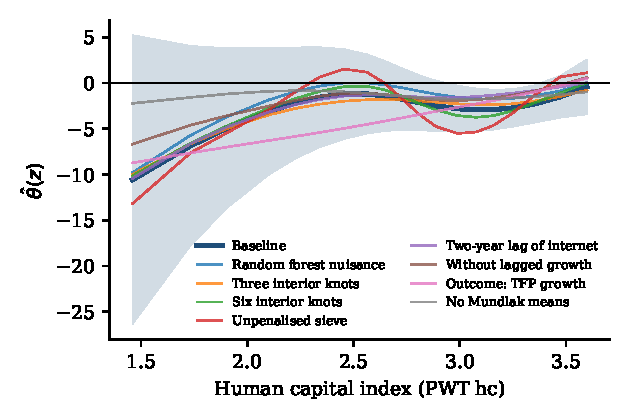
\includegraphics[width=\textwidth]{figures/emp_robust.pdf}
\caption{(a) $\hat\theta(z)$ by schooling across the WDI robustness checks that keep the baseline moderator, treatment and outcome (listed in Tables~\ref{tab:emp} and~\ref{tab:empappa}); three checks are highlighted and the shaded band is the 95\% pointwise band of the baseline. (b) $\hat\theta(z)$ by initial productivity in the WDI baseline, PWT 11.0 (1996--2023) and PWT 10.0 (1996--2019), with 95\% pointwise bands; the horizontal axis is the percentile of the moderator within each sample, because the levels are measured in different units (constant 2021 PPP dollars in WDI, current PPPs in 2021 and 2017 US dollars in PWT 11.0 and 10.0).}\label{fig:emprob}
\end{figure}

%% ===========================================================================
\clearpage
\section{Discussion}\label{sec:disc}

\subsection{Interpretation}

Three features of the results deserve emphasis. First, the estimated within-country association of lagged internet use with productivity growth is generally negative across the specifications considered, but its size is not robust. In the baseline, the 95\% interval excludes gains larger than $\nm{cihi}$ pp per year per ten points ($\nm{cihitw}$ with two-way clustering); this bound is specific to the baseline and its assumptions, and in several other specifications the interval includes zero. How negative the association is depends on what is held fixed: controlling for mobile and broadband subscriptions, which diffuse together with internet use, shrinks it towards zero. The literature suggests several explanations for a negative within-country association, which our design cannot distinguish: the J-curve argument that intangible investment and reorganisation depress measured productivity during diffusion \citep{brynjolfsson2021jcurve}, the concentration of ICT returns in firms with complementary capabilities \citep{gal2019digitalisation,nicoletti2020diffusion}, compositional effects in which digital platforms expand low-productivity service employment, and unobserved confounding. A negative within-country association is also consistent with a positive cross-country association in long differences, which reflects which economies adopted, not what adoption did within them.

Second, none of the heterogeneity predictions is supported robustly. With our precision, we cannot distinguish a flat function from moderate gradients of either sign, so the absence of evidence for complementarities with schooling is not evidence of their absence. Along initial productivity, some flexible fits suggest non-monotone variation, but the evidence is weak and not of the form the theories predict. The J-curve pattern along time since take-off that appeared in an earlier sample does not survive in the full sample.

Third, conclusions about where the digital dividend arrives are sensitive to the data. The gradient along initial productivity appears in both PWT releases and not in WDI data for the same countries and years. Within PWT, the revision of growth rates lowers the gradient on identical country-years, but the change is imprecisely estimated and depends on smoothing choices, which is itself a warning against reading such gradients as stable facts. These findings extend the evidence of \citet{johnson2013newer} and \citet{ponomareva2010pwt} on data revisions to heterogeneous associations of internet diffusion. They are not produced by the flexible estimator: they concern which data are used, and the estimator makes the uncertainty visible. The linear benchmarks point the other way in the WDI data: TWFE with a linear interaction gives a tercile contrast of $\nm{twgl}$ ($\nm{twglse}$) along initial productivity and TWFE with spline controls $\nm{twgs}$ ($\nm{twgsse}$). In the plasmode design without any effect, the same estimators produce gradients of similar size and reject in most replications (Table~\ref{tab:plasmodetwfe}), so we do not take this as evidence of a gradient.

\subsection{Policy implications}

Because the estimates are conditional associations, their policy content is limited, and they do not identify the return to connectivity investment. With that qualification, they caution against justifying connectivity programmes by expected short-run gains in aggregate measured productivity: in the economies and period we study, years with higher internet use were not followed by faster measured productivity growth within countries over horizons of up to nine years. This does not imply that such programmes are undesirable. Connectivity has consumer-surplus, inclusion and service-delivery benefits that productivity statistics do not capture \citep{worldbank2016wdr,goldfarb2019digital,hjort2025connectivity}, and averages across countries can hide large gains for specific groups within them. The literature offers several explanations for a missing aggregate pay-off that our data cannot test: gains may depend on complementary investment in firm capabilities, management and skills \citep{bloom2012americans,gal2019digitalisation}, on the intensity and quality of use rather than on access \citep{comin2018diffusion}, or on reorganisation that takes longer than our horizons \citep{brynjolfsson2021jcurve}. These are hypotheses for further work, not implications of our estimates. Finally, cross-country benchmarks that claim to identify the stage of development at which digital investment pays off should be treated with caution, because such heterogeneity estimates change with data releases. Policy-relevant causal statements would require designs with credible exogenous variation, such as the staggered arrival of infrastructure used by \citet{hjort2019internet}.

\subsection{Limitations}

The estimates are conditional associations of a lagged adoption level with growth, and the assumptions behind them are strong. Strict exogeneity rules out feedback from productivity shocks to future adoption; the lead test does not reject it but has little power, lagging the treatment by one or two years mitigates but does not eliminate reverse causality, and the instrument we could construct from historical fixed-line density is weak. Nuisance sufficiency requires that the controls and their country means capture the confounding path, which rules out, for example, global shocks with country-specific loadings that are correlated with adoption, or development trends that the controls do not track; region-by-year effects address the first concern only partly. The baseline avoids the mechanical violation of strict exogeneity that lagged productivity controls create, but other controls, such as urbanisation, may respond to past productivity, and convergence dynamics are absorbed only to the extent that initial productivity and the country means capture them. Measurement error matters in both directions: employment in low-income economies is largely modelled by the ILO and ITU internet shares for these economies are often estimated. In a linear model classical error in adoption would attenuate the coefficient; in our residualised varying-coefficient model the direction of the bias is not known in general. Results are similar with GDP-per-capita growth as the outcome, in countries with above-median statistical capacity, and without screening the adoption series, but they cannot rule out non-classical errors correlated with development. The last observations rest on provisional national accounts and schooling in 2024 is extrapolated. Internet penetration measures access, not intensity or quality of use. Coverage of low-income and conflict-affected economies is incomplete. Finally, the asymptotic theory covers the fixed-$K$ sieve with a vanishing penalty and, for the shape tests, a fixed penalty (Propositions~\ref{prop:an} and~\ref{prop:null}); the data-dependent penalty is evaluated by simulation only, and the bands describe the penalised fit rather than $\theta$ itself (Remark~\ref{rem:scope}).

%% ===========================================================================
\section{Conclusion}\label{sec:concl}

Over three decades of internet diffusion in 149 economies, we do not find a positive within-country association between lagged internet use and labour-productivity growth: in the baseline, a higher internet-user share is associated with slightly lower measured productivity growth, and the cumulative association remains negative over longer horizons, although its size depends on the specification. We find no robust variation of the association with schooling, initial productivity or time since take-off. Heterogeneity along the development dimension appears in the Penn World Table and not in World Bank data; within PWT, the revision of growth rates lowers it on identical country-years by an amount that we cannot distinguish from zero. These are conditional associations, not causal effects of connectivity.

Methodologically, Panel-DOSE combines orthogonal series estimation, Mundlak features, country-level cross-fitting, a within transformation and an O'Sullivan penalty, whose null space makes the constancy and linearity tests valid for a fixed penalty. In a plasmode design built on our data, the constancy test with the cross-validated penalty has close to nominal size for schooling and initial productivity but over-rejects for the skewed years-since-take-off moderator, so finite-sample calibration of this kind should accompany applications. In our simulations it is most useful when confounding is strongly nonlinear; when it is mild, TWFE with spline controls does as well. Most of its advantage comes from the Mundlak features, and linear interaction models give unreliable intervals when the control function is misspecified. The code, which also reports identifying variation, paired-bootstrap comparisons of estimates and shape tests, is released as a Python package.

Future work could combine the estimator with instruments or staggered infrastructure roll-outs to move from associations to effects, use firm- or region-level measures of the intensity of digital use, and examine the moderating roles of institutions, competition and data governance.

\section*{Data and code availability}
The data are publicly available from the World Bank's World Development Indicators (July 2026 release), the UNDP Human Development Report 2025 and the Penn World Table (versions 11.0 and 10.0). The WDI snapshot used here was retrieved through the World Bank API in September 2026 and is archived with SHA-256 checksums in the replication package, which reads the archived snapshot by default and verifies it before the panels are built. The package contains the Python implementation of Panel-DOSE, the scripts that reproduce all tables, figures and numbers in the text, and the list of package versions used.
\ifblind The package is available to the editor and reviewers; its location is given on the title page to preserve anonymity.\else The package is available at \url{https://github.com/vinhqdang/Journal-of-Digital-Economy}; an archived version with a persistent identifier will be deposited on acceptance.\fi

\ifblind\else
\section*{Declaration of competing interest}
The author declares no known competing financial interests or personal relationships that could have appeared to influence the work reported in this paper.

\section*{Funding}
This research did not receive any specific grant from funding agencies in the public, commercial, or not-for-profit sectors.

\section*{CRediT authorship contribution statement}
\textbf{Quang-Vinh Dang:} Conceptualization, Methodology, Software, Formal analysis, Data curation, Writing -- original draft, Writing -- review \& editing.
\fi

\bibliographystyle{elsarticle-harv}
\bibliography{refs}

\end{document}
